\ifdefined\ismainfile
    \def\GaugingProcedureEndDocument{}
\else
    \documentclass[11pt]{article}

    \makeatletter
\@ifclassloaded{revtex4-2}{}{\usepackage[margin=1in]{geometry}}
\makeatother
\usepackage{amsmath,amsthm,amsfonts,amssymb,mathrsfs}
\usepackage{graphicx}
\usepackage{cancel}
\usepackage{bm}
\usepackage{tikz}
\usepackage{csquotes}
\usepackage{tikz-3dplot}
\usepackage{physics}
\usepackage{dsfont}
\usepackage{float}
\usepackage{xcolor}
\usepackage{mathtools}
\usepackage{tcolorbox}
\makeatletter
\@ifclassloaded{revtex4-2}{\let\affil\affiliation
}{\usepackage{authblk}}
\makeatother

\tcbuselibrary{breakable}
\usepackage{keytheorems}
\newkeytheorem{definition}[parent=section, tcolorbox-no-titlebar={breakable, colback=blue!10}]
\newkeytheorem{example,lemma,conjecture,claim,theorem,proposition,corollary,fact,assumption,construction}[sibling=definition, tcolorbox-no-titlebar={breakable, colback=blue!10}]
\theoremstyle{definition}
\newtheorem{protocol}{Protocol}[section]

\newkeytheorem{remark}[parent=section, tcolorbox-no-titlebar={breakable}]
\allowdisplaybreaks[4]
\interdisplaylinepenalty=0
\makeatletter
\renewcommand{\log}{\mathop{\operator@font log}\nolimits}
\makeatother
\IfFileExists{bbm.sty}{\usepackage{bbm}}{\providecommand{\mathbbm}{\mathds}}
\usepackage{stmaryrd}
\usepackage{braket}
\makeatletter
\@ifpackageloaded{natbib}{}{\usepackage[numbers,sort&compress]{natbib}}
\makeatother
\usepackage{hyperref}
\usepackage[ruled,noline,longend]{algorithm2e}
\SetAlgoNoLine
\AtBeginDocument{\SetAlgoNoLine}
\SetAlgoLongEnd
\RestyleAlgo{boxruled}
\LinesNumbered
\definecolor{algcommentgray}{gray}{0.35}
\newcommand{\AlgCommentFont}[1]{\textcolor{algcommentgray}{#1}}
\SetCommentSty{AlgCommentFont}
\SetKwComment{tcp}{{\color{algcommentgray}$\blacktriangleright$}\ }{}
\usepackage{tcolorbox}
\tcbuselibrary{breakable}
\renewcommand{\topfraction}{0.9}
\renewcommand{\bottomfraction}{0.8}
\renewcommand{\textfraction}{0.07}
\renewcommand{\floatpagefraction}{0.85}
\setcounter{topnumber}{3}
\setcounter{totalnumber}{5}
\newenvironment{longalgorithm}[2][]{\begin{tcolorbox}[breakable, sharp corners, boxsep=0pt,
      boxrule=\algoheightrule, colframe=black, colback=white,
      left=18pt, right=4pt, top=5pt, bottom=5pt, #1]\refstepcounter{algocf}\noindent\hspace*{-14pt}{\textbf{\algorithmcfname~\thealgocf:} #2}\par
  \addcontentsline{loa}{algocf}{\protect\numberline{\thealgocf}#2}\par\nobreak\vspace{2pt}\nointerlineskip
  \moveleft18pt\vbox{\hrule width \dimexpr\linewidth+22pt\relax height \algoheightrule}\vspace{3pt}\setcounter{AlgoLine}{0}\RestyleAlgo{plain}}{\end{tcolorbox}}
\DontPrintSemicolon
\SetKwInput{KwIn}{Require}
\SetKwInput{KwOut}{Ensure}
\SetKwFor{For}{for}{do}{end for}
\SetKwFor{ForEach}{for each}{do}{end for}
\SetKwFor{While}{while}{do}{end while}
\makeatletter
\newenvironment{breakablealgorithm}{\par\addvspace{\intextsep}\hrule height .8pt\kern2pt
  \renewcommand{\caption}[2][]{\refstepcounter{algocf}\noindent\textbf{\algorithmcfname~\thealgocf:} ##2\par
    \kern2pt\hrule\kern2pt
    \ifx\relax##1\relax
      \addcontentsline{loa}{algocf}{\protect\numberline{\thealgocf}##2}\else
      \addcontentsline{loa}{algocf}{\protect\numberline{\thealgocf}##1}\fi
  }}{\par\kern2pt\hrule\addvspace{\intextsep}}
\makeatother
\usepackage{old-arrows}
\usepackage{color}
\usepackage{array, tabularx}
\usepackage{longtable}
\makeatletter
\@ifclassloaded{revtex4-2}{\appdef\@mkpream@relax{\let\@endpbox\relax}}{}
\makeatother
\usepackage{booktabs}
\newcolumntype{L}[1]{>{\raggedright\arraybackslash}p{#1}}
\newcolumntype{C}[1]{>{\centering\arraybackslash}p{#1}}
\newcolumntype{R}[1]{>{\raggedleft\arraybackslash}p{#1}}
\newcommand{\Circo}[0]{\mathfrak{C}}
\newcommand{\restrict}[2]{#1 \vert_{#2}}
\newcommand{\physq}[0]{\mathcal{M}}


\newcommand{\Xp}[0]{\mathcal{X}}
\newcommand{\Zp}[0]{\mathcal{Z}}

\newcommand{\nS}[1]{\mathbb{N}_{#1}}
\newcommand{\aS}[1]{\mathbb{C}_{#1}}

\newcommand{\nD}[1]{D^N_{#1}}
\newcommand{\aD}[1]{D^C_{#1}}

\newcommand{\control}[3]{C_{#1} {#2}_{#3}}
\usetikzlibrary{3d, shapes, arrows.meta, decorations.pathreplacing, decorations.markings, cd, shapes.geometric, calc}
\IfFileExists{tikzlibrarycalligraphy.code.tex}{\usetikzlibrary{calligraphy}}{}
\pgfkeysifdefined{/pgf/decoration/calligraphic brace/.@cmd}{}{\pgfkeys{/pgf/decoration/calligraphic brace/.style={brace}}}
\tikzstyle{midarrow} = [decoration={markings, mark= at position 0.6 with {\arrow{Stealth}}}, postaction={decorate}]
\renewcommand{\comment}[1]{{\color{red} #1}}

\newcommand{\YR}[1]{{\color{Teal} [Collin: #1]}}

\newcommand{\kc}[1]{{\color{cyan} [Katie: #1]}}

\newcommand{\bb}[1]{{\color{purple}[BB: #1]}}




\newcommand{\vva}[1]{{\color{magenta} [VVA: #1]}}









\newcommand{\al}[1]{{\color{DarkGreen} [Ana: #1]}}

\newcommand{\hp}[1]{{\color{brown} [Harry: #1]}}

\newcommand{\NT}[1]{{\color{orange} [NT: #1]}}

\newcommand{\dom}[1]{\textcolor{blue}{[Dom: #1]}}

\newcommand{\todo}[1]{\textcolor{blue}{[TO-DO: #1]}}

\newcommand{\new}[1]{{\color{DarkMagenta}#1}}
\definecolor{FGreen}{RGB}{58,158,92}
\definecolor{lightred}{RGB}{223, 123, 84}
\definecolor{lightbrown}{RGB}{242,216,199}
\definecolor{invisiblegray}{RGB}{238,238,237}
\definecolor{lightgreen}{RGB}{222, 235, 218}
\definecolor{lightcyan}{RGB}{153, 191, 216}
\definecolor{lightcyan2}{RGB}{208, 224, 235}
\definecolor{cyan2}{RGB}{144,201,226}
\definecolor{lightyellow}{RGB}{252, 238, 183}
\definecolor{OrangeRed}{RGB}{223,123,84}
\definecolor{CyanGreen}{RGB}{81,177,184}
\definecolor{rose}{RGB}{226,45,139}
\definecolor{Ycolor}{RGB}{248,236,104}
\definecolor{Hcolor}{RGB}{255,255,0}
\definecolor{Xcolor}{RGB}{246,143,138}
\definecolor{Zcolor}{RGB}{210,254,206}
\definecolor{Lred}{RGB}{244,163,163}
\definecolor{Lgreen}{RGB}{160,211,179}
\definecolor{Lblue}{RGB}{170,183,240}
\definecolor{tickcolor}{RGB}{181,0,250}
\definecolor{DarkBlue}{RGB}{14,38,80}
\definecolor{greenblue}{RGB}{0,255,127}
\definecolor{darkblue}{RGB}{57,85,134}
\definecolor{electrored}{RGB}{244,96,85}
\definecolor{electrored2}{RGB}{245,107,94}
\definecolor{BBXcheck}{RGB}{210,234,206}
\definecolor{BBZcheck}{RGB}{204,204,250}
\definecolor{softred}{RGB}{245,206,206}
\definecolor{fuchsiapurple}{RGB}{180, 0, 255}
\definecolor{Teal}{RGB}{62,138,141}
\definecolor{gold}{RGB}{233,168,58}
\definecolor{Crimson}{RGB}{220,20,60}
\definecolor{RedOrange}{RGB}{255,69,0}
\definecolor{DarkMagenta}{RGB}{139,0,139}
\definecolor{DarkGreen}{RGB}{0,100,0}
\definecolor{MidnightBlue}{RGB}{25,25,112}



\newcommand{\g}{\mathbf{g}}
\newcommand{\h}{\mathbf{h}}
\renewcommand{\k}{\mathbf{k}}
\newcommand{\f}{\mathbf{f}}
\newcommand{\C}{\mathbf{C}}
\newcommand{\Z}{\mathbb{Z}}
\renewcommand{\S}{\mathcal{S}}
\newcommand{\CC}{\mathcal{C}}
\newcommand{\charge}{k}
\newcommand{\totalcharge}{K}
\newcommand{\B}{\mathbb{B}}
\renewcommand{\O}{\mathcal{O}}
\newcommand{\Ocal}{\mathcal{O}}
\renewcommand{\Vec}{\mathcal{V}ec}
\newcommand{\Rep}{\text{Rep}}
\newcommand{\nnb}{\nonumber}
\newcommand{\lt}{\triangleleft}
\newcommand{\rt}{\triangleright}
\newcommand{\Lcal}{\mathcal{L}}
\newcommand{\Acal}{\mathcal{A}}
\newcommand{\Gcal}{\mathcal{G}}
\newcommand{\XX}{\mathcal{X}}
\newcommand{\YY}{\mathcal{Y}}
\newcommand{\ZZ}{\mathcal{Z}}
\newcommand{\Com}[2]{[ #1, #2 ]}
\newcommand{\ComGrp}[2]{[ #1, #2 ]_{\text{grp}}}
\newcommand{\level}{\operatorname{Lv}}
\newcommand{\code}{\mathcal{C}}


\newcommand{\glosym}[0]{\mathsf{L}}
\newcommand{\im}{\operatorname{im}}
\newcommand{\rk}{\operatorname{rk}}
\newcommand{\supp}[1]{\operatorname{Supp}(#1)}
\newcommand{\Ad}{\operatorname{Ad}}
\newcommand{\Irrep}{\operatorname{Irrep}}
\newcommand{\Wt}{\operatorname{Wt}}
\newcommand{\Lin}{\mathfrak{L}}
\newcommand{\interior}{\operatorname{int}}
\newcommand{\T}[0]{\mathsf{U}}
\newcommand{\orbit}[1]{O^{\mathcal{T}}(#1)}
\newcommand{\sym}[0]{\overline{S}}
\newcommand{\av}[0]{\mathbb{A}_v}
\newcommand{\bp}[0]{\mathbb{B}_f}
\newcommand{\onsite}[1]{\mathsf{T}|_{#1}}
\newcommand{\Log}[1]{\overline{#1}}
\newcommand{\id}[0]{\mathbf{1}}
\newcommand{\bd}[1]{\delta({#1})}
\newcommand{\zp}[0]{\mathbb{Z}_p}
\newcommand{\cX}[0]{\mathcal{X}}
\newcommand{\cZ}[0]{\mathcal{Z}}
\newcommand{\cC}[0]{\mathcal{C}}
\newcommand{\cE}[0]{\mathcal{E}}
\newcommand{\cx}[2]{CX_{#1\rightarrow#2}}
\newcommand{\wcp}[2]{\mathcal{C}P_{#1\rightarrow#2}}
\newcommand{\wcx}[2]{\mathcal{C}X_{#1\rightarrow#2}}
\newcommand{\wcz}[2]{\mathcal{C}Z_{#1\rightarrow#2}}
\newcommand{\wcy}[2]{\mathcal{C}Y_{#1\rightarrow#2}}
\newcommand{\cpw}[2]{C\mathcal{P}_{#1\rightarrow#2}}
\newcommand{\cxw}[2]{C\mathcal{X}_{#1\rightarrow#2}}
\newcommand{\czw}[2]{C\mathcal{Z}_{#1\rightarrow#2}}
\newcommand{\cyw}[2]{C\mathcal{Y}_{#1\rightarrow#2}}
\newcommand{\wct}[2]{\mathcal{C}\mathcal{T}_{#1\rightarrow#2}}
\newcommand{\wctdag}[2]{\mathcal{C}\mathcal{T}^\dagger_{#1\rightarrow#2}}
\newcommand{\cnot}[0]{\CNOT}
\newcommand{\SWAP}[0]{\mathsf{SWAP}}
\newcommand{\CNOT}[0]{\mathsf{CNOT}}
\newcommand{\CSWAP}[0]{\mathsf{CSWAP}}
\newcommand{\CX}[0]{\mathsf{CX}}
\newcommand{\CZ}[0]{\mathsf{CZ}}
\newcommand{\CT}[0]{\mathsf{CU}}
\newcommand{\swap}[0]{\SWAP}
\newcommand{\cswap}[0]{\CSWAP}

\newcommand{\overlap}[1]{\Omega(#1)}
\newcommand{\E}[2]{e_{(#1,#2)}}
\newcommand{\dec}[1]{\tilde{#1}}
\newcommand{\insuppof}[2]{#1|_{#2}}
\newcommand{\plushalf}[1]{{#1+\frac{1}{2}}}
\newcommand{\minushalf}[1]{{#1-\frac{1}{2}}}
\newcommand{\scrG}[0]{{\mathscr{G}}}
\newcommand{\sset}[1]{\Sigma(#1)}

\newcommand{\symOP}{\T}
\newcommand{\symS}{\overline{S}}
\newcommand{\haH}{\mathsf{H}}
\newcommand{\haA}{\mathsf{A}}
\newcommand{\haB}{\mathsf{B}}
\newcommand{\haP}{\mathsf{P}}
\newcommand{\haQ}{\mathsf{Q}}
\newcommand{\haX}{\mathsf{X}}
\newcommand{\Deco}{\mathfrak{D}}

\newcommand{\vertexset}[1]{\Sigma^{-1}(#1)}
\newcommand{\invvertexset}[1]{\Sigma(#1)}
\newcommand{\faceP}{\mathcal{P}} 
\newcommand{\vertexV}{\mathsf{V}}
\newcommand{\edgeE}{\mathsf{E}}
\newcommand{\faceF}{\mathsf{F}}
\newcommand{\graphG}{\mathsf{G}}
\newcommand{\intG}{\mathbb{G}}
\newcommand{\N}{\mathsf{N}}
\newcommand{\eigenE}{\mathbf{E}} 
\newcommand{\gaugedA}{\mathbb{A}}
\newcommand{\gaugedB}{\mathbb{B}}
\newcommand{\gaugedS}{\mathbb{S}}
\newcommand{\Sdec}{\mathfrak{s}}
\providecommand{\vr}{}
\renewcommand{\vr}{v_r}
\newcommand{\gaugedH}{\mathbb{H}}
\newcommand{\gaugingOP}{\mathscr{G}}
\newcommand{\chproj}[2]{\llbracket #1\rrbracket _{#2}}

\newcommand{\gX}{\mathcal{X}}
\newcommand{\gZ}{\mathcal{Z}}
\newcommand{\mX}{\mathcal{X}}
\newcommand{\mZ}{\mathcal{Z}}
\newcommand{\gW}{\mathcal{W}}
\newcommand{\gY}{\mathcal{Y}}
\newcommand{\Agrp}{\mathbf{A}}
\newcommand{\chOmega}{\mathit{\Omega}}
\newcommand{\Linex}{\Lin_{\rm ex}(\mathcal H_{\rm m})}
\newcommand{\Linnt}{\Lin_{\rm nt}^{\rm ex}(\mathcal H_{\rm mat})}


\newcommand{\K}{\mathcal{K}}
\newcommand{\gaugedT}{\mathbb{T}}
\newcommand{\Stab}{\mathcal{G}}
\newcommand{\F}{\mathcal{F}}
\newcommand{\Hp}{\mathcal{H}}
\newcommand{\Poly}{\mathsf{Poly}}
\newcommand{\Fphys}{F_{\text{phys}}}
\newcommand{\Fmeas}{F_{\text{meas}}}
\newcommand{\Fp}{\mathbf{F}_p}
\newcommand{\Zq}{\mathbb{Z}_q}
\newcommand{\Sprod}[2]{\Lambda\left( #1, #2 \right)}
\newcommand{\FT}{F^T}
\newcommand{\nbhd}{\mathsf{N}}

\newcommand{\Cgeom}{C_{\text{geom}}}
\newcommand{\CLDPC}{C_{\text{LDPC}}}
\newcommand{\Cstep}{C_{\text{step}}}
\newcommand{\Cretract}{C_{\text{retract}}}
\newcommand{\Ctotal}{C_{\text{total}}}
\newcommand{\Cgauge}{C_{\text{gauge}}}

\newcommand{\nonabel}[1]{S^\mathrm{N}_{#1}}
\newcommand{\abel}[1]{S^\mathrm{A}_{#1}}
\newcommand{\gnonabel}[1]{\mathbb{S}^\mathrm{N}_{#1}}
\newcommand{\gabel}[1]{\mathbb{S}^\mathrm{A}_{#1}}
\newcommand{\onset}[2]{{#1}_{\sset{#2}}}
\newcommand{\ccomm}[2]{[#1,#2]_{\mathrm{grp}}}
\newcommand{\tu}[0]{t_{\mathrm{u}}}
\newcommand{\tg}[0]{t_{\mathrm{g}}}
\newcommand{\tf}[0]{t_\mathrm{f}}
\newcommand{\Ig}[0]{\mathrm{I}_{\mathrm{g}}}
\newcommand{\Ifn}[0]{\mathrm{I}_\mathrm{f}}
\newcommand{\Ib}[0]{\mathrm{I}_0}
\newcommand{\cA}[0]{\mathcal{A}}
\newcommand{\cQ}[0]{\mathcal{Q}}
\newcommand{\cK}[0]{\mathcal{K}}
\newcommand{\grpcom}[2]{\ComGrp{#1}{#2}}
\newcommand{\de}[0]{d_\mathcal{E}}



\definecolor{Teal}{RGB}{0,128,128}
\definecolor{Crimson}{RGB}{220,20,60}
\definecolor{RedOrange}{RGB}{255,69,0}
\definecolor{DarkMagenta}{RGB}{139,0,139}
\definecolor{DarkGreen}{RGB}{0,100,0}
\definecolor{MidnightBlue}{RGB}{25,25,112}


\hypersetup{
    colorlinks=true,
    linkcolor=MidnightBlue,
    citecolor=MidnightBlue,
    urlcolor=MidnightBlue,}

\usepackage{amsfonts,latexsym,amsthm,amssymb,amsmath,amscd,euscript,tikz,mathtools}
\usepackage{framed}
\usepackage[normalem]{ulem}
\makeatletter
\@ifclassloaded{revtex4-2}{}{\usepackage[margin=1in]{geometry}}
\makeatother
\usepackage{color}




\usepackage{enumitem}
\usepackage{environ}
\usepackage{dcolumn}

\usetikzlibrary{positioning, shadows, arrows, backgrounds, fit}
\usetikzlibrary{decorations.pathmorphing}

\definecolor{Teal}{RGB}{0,128,128}

\hypersetup{
    colorlinks=true,
    linkcolor=MidnightBlue,
    citecolor=MidnightBlue,
    urlcolor=MidnightBlue,
}

\definecolor{GrayOut}{gray}{0.8}
\NewEnviron{GrayedOut}{\begingroup\color{GrayOut}\BODY\endgroup
}

\newcommand{\diam}{\operatorname{diam}}
\newcommand{\dist}{\operatorname{dist}}

\newcommand{\cH}{\mathcal{H}}
\newcommand{\cT}{\mathcal{T}}
\newcommand{\cN}{\mathcal{N}}
\newcommand{\cB}{\mathcal{B}}
\newcommand{\bbP}{\mathbb{P}}
\newcommand{\haT}{\mathsf{T}}
\newcommand{\haD}{\mathsf{D}}
\newcommand{\cF}{\mathcal{F}}

\newcommand{\CZero}{C_0(\Gcal_0)}
\newcommand{\COne}{C_1(\Gcal_1)}
\newcommand{\deltaOne}{\delta_1}
\newcommand{\jall}{\mathbf{1}}
\newcommand{\tof}[0]{\ket{\mathsf{Tof}}}
\newcommand{\Pp}[1]{\mathrm{P}^+_{\Log{#1}}}
\newcommand{\Ppk}[1]{\mathrm{P}^+_{\Log{#1}^{\otimes k}}}
\newcommand{\Pm}[1]{\mathrm{P}^-_{\Log{#1}}}

\newcommand{\fa}[0]{F_\mathrm{A}}
\newcommand{\fn}[0]{F_\mathrm{N}}

\newcommand{\CHANGE}[1]{{\color{DarkMagenta}#1}}

\newcommand{\syndromeSet}{\sigma}
\newtheorem{axiom}{Axiom}[section]
\newtheorem{question}{Question}[section]


\newcommand{\green}[1]{\textcolor{Teal}{#1}}
\newcommand{\blue}[1]{\textcolor{blue}{#1}}
\newcommand{\red}[1]{\textcolor{red}{#1}}

\makeatletter
\let\UncappedLeft\left
\let\UncappedRight\right
\def\left{\@ifnextchar({\CappedLeftParen}{\UncappedLeft}}
\def\CappedLeftParen(#1\right{\@ifnextchar){\CappedRightParen{#1}}{\UncappedLeft(#1\UncappedRight}}
\def\CappedRightParen#1){\mathopen{}\bigg(#1\bigg)\mathclose{}}
\makeatother

\definecolor{vred}{rgb}{0.85,0,0}
\definecolor{epur}{cmyk}{0.45,0.86,0,0}
\definecolor{poraBase}{cmyk}{0,0.42,1,0}
\colorlet{pora}{poraBase!90!black}
\definecolor{setgray}{RGB}{225,225,225}
\newcommand{\vC}[1]{{\color{vred}#1}}
\newcommand{\eC}[1]{{\color{epur}#1}}
\newcommand{\pC}[1]{{\color{pora}#1}}
\newcommand{\sq}[9]{\left(\begin{smallmatrix}
\vC{#1} & \eC{#2} & \vC{#3}\\[1pt]
\eC{#4} & #5 & \eC{#6}\\[1pt]
\vC{#7} & \eC{#8} & \vC{#9}
\end{smallmatrix}\right)}
\newcommand{\mm}[4]{\begin{smallmatrix}#1 & #2\\ #3 & #4\end{smallmatrix}}
\newcommand{\sqe}[5]{\sq{\cdot}{#1}{\cdot}{#2}{#3}{#4}{\cdot}{#5}{\cdot}}
\newcommand{\Sg}{\mathsf{S}}
\newcommand{\CZbar}{\overline{CZ}}

\setcounter{tocdepth}{1}

    
    \begin{document}
    \title{Procedure for measuring logical Clifford operators}
    \date{\today}

    \maketitle
    \def\GaugingProcedureEndDocument{\end{document}}
\fi

  
In this section, we describe how to implement a gauging measurement of a Clifford operator~$\T$. Starting with an LDPC code possessing a transversal logical Clifford operator, we can systematically produce a deformed---``gauged''--- LDPC code that contains $\T$ in its stabilizer group. The value of $\T$ can be inferred from the syndrome outcomes of the gauged code, and the system is left in an eigenstate of $\T$ after returning to the original code. We present some explicit examples of the application of our method in Sec.~\ref{sec:examples}. The reader that is not interested in the technical proofs of either the gauged code distance or the fault tolerance of the gauging measurement may proceed directly to Sec.~\ref{sec:examples} after this section.



We begin by enumerating the requirements on the initial code and its transversal gate, followed by the necessary properties of the ancilla system we  use to perform the gauging procedure. Then we write down the explicit gauging circuit (Definition \ref{def:gauging-circuit}). We demonstrate the action of this circuit through an explicit example: gauging $\CZbar$ on the $[[4, 2, 2]]$ code. Then, we derive closed-form expressions for the gauged code stabilizers for two cases: (i) an initial qubit stabilizer code and transversal gate $\T$ such that $\T^2 = \id$, and (ii) a generic qudit code with $\T^p = \id$ for some integer $p$.

\subsection{Gauging measurement protocol}\label{subsec:gauging-protocol}
We start with an LDPC code $\cC = \langle S_i \rangle$ and unitary transversal gate. 

\begin{definition}[Transversal Gate] \label{def:transversal-gate}
    A transversal gate $\T$ acting on a code $\cC$ with a set of qubits $\physq$ is a finite-depth circuit taking the following form:
\begin{equation}
    \T = \otimes_{v \subset \physq} \T_{v}, \quad \bigcup_v v = \physq, \quad v \cap v' = \emptyset
    \label{eq:block-form}
\end{equation}
where each $v$ is an $O(1)$ subset of the code qubits, and $\T_{v}$ is a unitary acting solely on this subset. 
\end{definition}
We note that if we set $k = \max_{v} |v|$, this definition is equivalent to a $k$-fold transversal gate as defined in \cite{chakraborty2026}.


In general, we may have a qudit code with qudits of dimension $q$ and a transversal gate with order $p$: $\T^p = \id$. We also assume that $\T_{v}^p = \id$ for all $\T_{v}$.\footnote{This is always possible via the introduction of local phases multiplying the $\T_{v}$ that cancel on the full transversal gate $\T$.} We act on qudits with clock and shift operators, $X$, $Z$:

\begin{align}
    ZX = \omega XZ, &\quad \omega = e^{2\pi i/q} \\
    X^q = &Z^q = \id
\end{align} When $q=2$, we recover the usual Pauli algebra.  

Since $p \neq q$ in general, and we need to introduce ancilla qudits of dimension $p$ to perform the gauging measurement, we distinguish clock and shift operators acting on these local degrees of freedom of dimension $p$ with a different font; $\cX,\cZ$ with $\cX^p = \cZ^p = \id$ and $\cZ \cX = \Omega \cX \cZ$ for phase $\Omega = e^{2\pi i/p} $. In the condensed matter literature, it is common to refer to the degrees of freedom of the initial LDPC code as \textit{matter} qudits, and the ancilla qudits as \textit{gauge} qudits. The states $\ket{+}$ and $\ket{0}$ denote the $+1$ eigenstates of the qudit shift and clock operators respectively, with the dimension of the qudit understood from context.

We write the support of an operator $O$ restricted to some subset $A$ of the physical degrees of freedom as $O_A$. We frequently make use of the group commutator: $\ComGrp{A}{B} = A B A^\dagger B^\dagger$. Finally, we denote a controlled-$U$ gate with control $a$ and target $b$ as follows:
\begin{equation}
    \control{a}{U}{b} = \control{a}{(U)}{b} \equiv \sum_{n = 0}^{d_a - 1} \dyad{n}_a \otimes U^{n}_b
\end{equation} where $d_a$ is the dimension of the control qudit $a$.\footnote{Note that this gate is a unitary only when the order of $U$ divides $d_a$. However, in the case considered here, we have $d_a = p$ and $U = \T_v$, and as such this gate is always unitary.}


We now provide a conceptual overview of the gauging protocol. We aim to measure a logical Clifford operator $\T$--- perhaps to prepare a magic state, or implement a logical gate teleportation scheme--- and we wish to do it in a fault-tolerant manner. By gauging the logical Clifford, we map our initial code $\cC$ onto a deformed code $\cC'$ with $\T$ in its stabilizer group. If this deformed code $\cC'$ is itself a QLDPC code (not, however, a Pauli stabilizer code), we can convert the measurement of $\T$ into the measurement of constant weight stabilizer generators instead.

\begin{definition}[Gauging the logical operator of a quantum code]
    Take a code $\cC$ and a transversal logical gate $\T$ satisfying $\T^p = \id$. Let the codespace of the \emph{symmetric code} be the intersection of the codespace of $ \cC $ and the $+1$ eigenspace of $\T$. This is, in general, a non-LDPC code, because $\T$ may act on extensively many qu(d)its. \emph{Gauging} maps the codespace of a symmetric code to an isomorphic codespace belonging to a QLDPC code, $\cC'$ called the \emph{gauged} code.
\end{definition}



The following section describes how to arrive at the generators of the gauged QLDPC code $\cC'$.
We first introduce an auxiliary connected graph $\graphG=(\vertexV,\edgeE)$ whose vertices are identified with the local gates $\T_{v}$. The properties of the graph influence the fault tolerance of the procedure. 
Since $\T$ may have extensive weight, and our goal is to measure it in a fault-tolerant way, we introduce new constant-weight operators $\av$ such that
\begin{equation}
    \prod_v \av = \T,
    \label{eq:gauged-sym}
\end{equation} 
where $\av=\T_v \prod_{e\in \delta v} \Xp_e$, and $\delta: \vertexV \to \edgeE$ is the coboundary map of $\graphG$. The introduction of these new operators allows us to break up the measurement of a large operator into small pieces, since measuring the $\av$ also measures $\T$. This measurement could be used to prepare a magic state or drive a measurement-based logic gate.

\begin{definition}[Gauging Measurement Protocol]
\label{def:gauging-measurement-protocol}
    The gauging measurement for a transversal logical operator $\T$ with $\T^p = \id$ is described by a simple procedure~\cite{williamson2024lowoverheadfaulttolerantquantumcomputation}:

\begin{enumerate}
    \item Initialize an auxiliary qudit of dimension $p$ in the state $\ket{0}_e$ for each edge $e\in \edgeE$.
    \item Measure all $\av$ operators.
    \item Measure all $\Zp_e$ operators. 
    \item Apply a feedforward operation of the form $\prod_{v} \T^{a_v}_v$ for some subset of the vertices $\{v\} \subseteq \vertexV$ and some set of $a_v \in \{0, \dots, p-1\}$.
\end{enumerate} 
\end{definition}
The above procedure can be applied to any operator $\T$ that satisfies $[\T_v,\T_{v'}]=0$ for all $v,v'\in \vertexV$. For simplicity, we focus on transversal gates $\T$ where each $\T_v$ is supported on a distinct, tensor factor (with $O(1)$ support).




The gauging measurement protocol implements the projective measurement of the target gate~$\T$. 
\begin{lemma}[Gauging measurement operation~\cite{williamson2024lowoverheadfaulttolerantquantumcomputation}]  
Let $a_v$ denote the measurement outcome of $\av$ in the gauging measurement protocol of Def.~\ref{def:gauging-measurement-protocol}.
This protocol performs a projective measurement of the symmetry $\T$ with outcome 
\[
\sigma = \prod_{v\in \vertexV} a_v .
\]
Equivalently, up to the feedforward operation in Def.~\ref{def:gauging-measurement-protocol}, the final state on the original code is given by: 
\[
\Pi_\sigma \ket{\psi_\mathrm{initial}}, \quad \Pi_\sigma = \frac{1}{p} \sum_{a=0}^{p-1} \sigma^{-a} \T^a.
\]
\end{lemma}
\begin{proof}
The proof is given in Ref.~\cite{williamson2024lowoverheadfaulttolerantquantumcomputation}, and the argument is discussed in Sec. \ref{sec:ungauging}.
\end{proof}

In general, the stabilizers of the original, ungauged code $\cC$ do not commute with each $\av$. As a result, after step~2, the code is deformed into a \textit{gauged code} $\cC'$. The gauged code has additional checks $\av$ and $\bp:=\prod_{e\in \partial p} \cZ_e$ where $\partial p$ form a cycle basis of $\graphG$. The original checks $S_i$ of code $\cC$ are updated into \emph{decorated stabilizers} $\gaugedS_i$ which are modified to ensure that they commute with the added $\av$ and $\bp$ operators in the codespace. Our goal is to construct a graph $\graphG$ such that the deformed code $\cC' = \langle \gaugedS_i, \av, \bp \rangle$ retains a high distance, and remains an LDPC code. We discuss the necessary properties of $\graphG$ in Sec. \ref{sec:defining-gauging-graph}.

We now consider a circuit-level implementation of steps 1 and 2 of Definition~\ref{def:gauging-measurement-protocol}. 
Given a suitable choice of gauging graph $\graphG$, we can write down the stabilizers of the gauged code in a systematic way:


\begin{enumerate}
    \item \textbf{Define vertex sets:} Break the support of the transversal gate $\T$ into \emph{vertex sets}. These are constant-sized subsets of the original code degrees of freedom which form a partition of the support of $\T$. This choice of subsets defines a map $\Sigma: \physq \to \vertexV$ from matter qudits to their corresponding vertex set $v \in \vertexV$. The minimal choice for a vertex set is the ``unit cell'' of the $\T$ action. For example, consider a transversal gate made up of single-qudit gates that acts identically on all qudits. A straightforward choice of partition is to make each matter qudit a distinct vertex set. We discuss how to choose vertex sets in more detail later in Sec. \ref{sec:defining-gauging-graph}.
    
    \item \textbf{Add vertex ancilla qudits (symmetry enrichment):} We add a \emph{vertex ancilla} for each vertex set $v \in \vertexV$, initialized in the state $\ket{+}_v$ (add stabilizers $\Xp_v$). The pre-image $\vertexset{v} \subseteq \physq$ gives the set of all matter qudits associated to a given vertex set/ancilla. Let $\T_v:=\T_{\vertexset{v}}$ denote the local factor of the transversal gate supported on $\vertexset{v}$; in general $\T_v$ may be a multi-qudit operator. Apply controlled gates to each vertex set that perform the following basis transformation: $$\Xp_v \xrightarrow {C_v \T_v}\Xp_v \T_v.$$ At this point, our wavefunction is a $+1$ eigenstate of $\T \otimes \prod_v \Xp_v$ (this is the product of all the newly added stabilizers).
    
    \item \textbf{Add edge ancilla qudits (cluster state entangler):} We aim to generate a state that is an eigenstate of $\T$ by itself, not of some joint operator on the matter qudits and the ancilla degrees of freedom. We want a circuit that takes $\prod_v \Xp_v \to \id$. To do this, we introduce a second set of \emph{edge} ancillas, $\edgeE$, each initialized in the $\ket{0}$ state. As suggested by the notation, we define the oriented graph $\graphG = (\vertexV, \edgeE)$---called the \emph{gauging graph}--- on which these edge ancillas live shortly. We apply a graph cluster state entangler between the vertex and edge ancilla, which performs the following basis transformation: $$\Xp_v \T_v \xrightarrow{\text{cluster entangler}} \Xp_v \T_v \prod_{e \in \delta v} \Xp^{\eta_v(e)}_e.$$ Here, $\eta_v(e) \in \{-1, 1\}$ is a function giving the orientation of an edge $e$ with respect to vertex~$v$.
    
    \item \textbf{Measuring out vertex ancillas:} Finally, we complete the gauging process by measuring out the vertex ancillas in the $\Xp$ basis, producing the desired $\av$ stabilizers, up to a phase: $$\av = \omega^{m_v} \T_v \prod_{e \in \delta v} \Xp^{\eta_v(e)}_e, \quad \omega = e^{2\pi i /p}.$$ 
    Here, $m_v \in \{0, \dots, p-1\}$ denotes the measurement outcome for $\Xp_v$. We can always apply a finite-depth circuit to correct all $m_v \neq 0$ outcomes to $m_v = 0$ \cite{Tantivasadakarn_2023, Ren_2025}. 
    Once corrected, the product of all these $\av$ terms is simply $\T$, since each edge $e$ on the gauging graph is shared by two vertices and the $\eta$ function ensures one vertex contributes $\Xp$ while the other contributes $\Xp^\dagger$. At this point we have successfully implemented the measurement of $\T$.
\end{enumerate}

Collected into a single expression, the above protocol is as follows: 


\begin{definition}[Gauging Map (Circuit-Level)] \label{def:gauging-circuit}
Consider a code $\cC$ and associated transversal gate $\T$. Given a choice of vertex set (the map $\Sigma$) and gauging graph $\graphG = (\vertexV, \edgeE)$ with edge orientations given by $\eta_v(e)$, the gauging operation taking $\cC \to \cC'$ is implemented by the following three-part map $\tilde{\Gamma}$:
\begin{equation}
\widetilde{\Gamma} \equiv  \underbrace{\left (\prod_{v \in \vertexV} \dyad{+}_v \right )}_\textrm{P} \underbrace{\left ( \prod_{v \in \vertexV} \prod_{e \in \delta v} C_v \Xp^{\eta_v(e)}_e \right )}_{\textrm{C.E.}} \underbrace{\left ( \prod_{v \in \vertexV} C_v \T_v \right )}_\textrm{S.E.} \underbrace{\left ( \prod_{v \in \vertexV} \ket{+}_v \prod_{e \in \edgeE} \ket{0}_e \right )}_\textrm{Ancilla Init.}
    \label{eq:gauging-circuit}
\end{equation}

The labels for each part of the map stand for (0) ``Ancilla Initialization'', which we will normally take as given, (1) ``Symmetry Enrichment'', (2) ``Cluster Entangler'', and (3) ``Projection''. In practice, the final projection is implemented by an adaptive circuit consisting of measurement in the $\Xp$ basis on the vertex ancilla and feedback to correct erroneous ($\neq + 1$) measurement outcomes.
\end{definition}

In the following sections we describe each of these steps in more detail, and derive the general form for the resultant gauged code stabilizers. We note that our procedure builds on Refs.~\cite{Williamson_2021,verresen2022efficientlypreparingschrodingerscat,Tantivasadakarn_2023,Tantivasadakarn_2024,Ren_2025}, where the gauging circuit was developed for topological codes. The protocol presented here applies to any qudit LDPC stabilizer code and any suitable transversal gate $\T$.

\subsection{Defining the gauging ancilla system} \label{sec:defining-gauging-graph}




We now consider the design of the gauging graph. The first step is to pick the vertices $\vertexV$ of the gauging graph. We start with a code $\cC$ and a transversal gate of interest, $\T$. We then aim to choose a map $\Sigma: \physq \to \vertexV$ that satisfies the conditions below. 

\begin{enumerate}
    \item \textbf{Constant size:} We want to ensure that the gauged code $\cC'$ remains LDPC; this implies that we must have $|\vertexset{v}| \sim O(1)$ for all $v \in \vertexV$, or else the $\av$ terms may not be LDPC.
    \item \textbf{No overlap:} We also require that $\Sigma$ is a valid function: i.e. each physical qudit belongs to exactly one vertex set. This partition should respect the structure of $\T$, meaning the support of an elementary gate of $\T$ should not be split across vertex sets. As mentioned above, a minimal choice of vertex set for a single-qubit strongly transversal gate would be one qudit per vertex set. By contrast, a transversal $\CNOT$ acting between two codeblocks naturally lends itself to vertex sets consisting of one qubit from each codeblock, since a single qudit vertex set would not contain the full support of a single $\CNOT$. 
\end{enumerate}


Assuming we have satisfied these constraints, there are many valid choices for $\Sigma$. The particular structure of a given starting code $\cC$ informs the most convenient vertex set--- for instance, a good choice for code living on a tri-colorable lattice may be to make faces of a certain color vertex sets. We present such examples below. In general, however, we can always pick the ``minimal'' choice of vertex set, dependent on the structure of the transversal gate $\T$ itself.


\begin{definition}[Minimal Vertex Set]
Given a transversal gate $\T$ acting on a code $\cC$ with the form given in Def. \ref{def:transversal-gate}, the \emph{minimal vertex set} is chosen such that each vertex ancilla $v$ corresponds to a minimal local action $\T_v \subset \T$. In other words, no $\T_v$ can be written as a tensor product supported on a smaller subset of qudits.
\end{definition}

\begin{definition}[Valid Vertex Set]
    A \emph{valid vertex set} is any coarse-graining of the minimal vertex set (where coarse-graining merges some vertex sets into one larger vertex set).  
\end{definition}


We complete the specification of the graph $\graphG$ by adding edges connecting vertices $\vertexV$. These edges are required to obey certain restrictions to produce a valid gauging measurement protocol. Again, we want to ensure that the final code $\cC'$ is LDPC, which enforces that $\graphG$ should have $O(1)$ degree--- otherwise, the $\av$ operators may not be low-weight. We also require that $\graphG$ has a sparse cycle basis: we show below that the gauging protocol produces new stabilizers $\bp$ for every cycle of $\graphG$, and a sparse cycle basis ensures there is a generating set of $\bp$ that are LDPC. The last condition that ensures the gauged code is LDPC is a ``well-connected'' condition, which ensures any modifications to the original stabilizers are LDPC as well. To ensure we measure only $\T$ and not individual operators whose product is $\T$, we want $\graphG$ to consist of a single connected component. Finally, to ensure the code $\cC'$ has the same distance scaling as the code $\cC$, we want the homology of $\cC'$ to be completely determined by $\cC$, and thus $\graphG$ should be homologically trivial (this is actually already satisfied if we have specified a complete, sparse cycle basis).
We collect these constraints into a set of desiderata, below. 



\begin{definition}[Graph Desiderata] \label{def:graph-desiderata}
When constructing the gauging graph $\graphG$, the following suffice to ensure a well-behaved gauged code.


\begin{enumerate}

\item \textbf{Connectedness:} $\graphG$ should be connected to ensure the desired logical action.

\item \textbf{Sparseness:}
\begin{enumerate}
    \item \emph{Bounded degree.} The degree of $\graphG$ should be bounded by a constant.
    \item \emph{Sparse cycle filling.} Each 2-cell $p\in\graphG_2$ has a boundary $\partial_2p$ of uniformly $O(1)$-bounded weight. Equivalently, $\supp{\gaugedB_p}$ is bounded by some constant for all $p$. This can be ensured by applying a decongestion procedure to $\graphG$ as described in Refs.~\cite{williamson2024lowoverheadfaulttolerantquantumcomputation,swaroop2025universaladaptersquantumldpc,yuan2026parsimonious}. 
    \item \emph{Well-connected.} Any pair of vertices whose corresponding vertex sets share support on at least one stabilizer are connected by a path that contains a constant number of edges. This is required to ensure the gauged code is LDPC.
\end{enumerate}

\item \textbf{Distance preserving:}
    \begin{enumerate}
        \item \emph{Trivial homology.} When the gauging graph is expressed as a chain complex (see Def. \ref{def:gauging-complex}), the homology $H_1$ should be trivial. This ensures that no additional, potentially low-weight, diagonal logical operators are introduced on the edge qudits. Enforcing a sparse cycle basis also ensures this condition.
        \item \emph{Expansion.} The generalized Cheeger constant of $\graphG$ (see Def.~\ref{def:generalized-cheeger})  should satisfy
        \[
        h_{\Agrp}(\graphG)\ge 1.
        \]
        This condition is only required before cycle decongestion. 
    \end{enumerate}
\end{enumerate}
    
\end{definition}

A straightforward choice of $\graphG$, given these constraints, is the following: place an edge between any two vertex ancillas whose associated vertex sets have support on the same stabilizer.


For each stabilizer $S \in C$ define an edge $e = (v, v') \in \edgeE$ for any pair $v, v' \in \invvertexset{\supp{S}}$, where $\supp{S}$ denotes the qudits in the support of the stabilizer $S$. The LDPC property of the input code ensures that the resulting graph is sparse.
We remark that this choice is somewhat redundant, as it suffices to include a spanning tree on the vertices in the support of any stabilizer to ensure the well-connected property. Furthermore, this choice does not suffice to guarantee connectedness or sufficient expansion. These properties can be guaranteed by adding further edges, such as those of an expander graph. 


\begin{lemma}[Construction of a suitable graph]
We can always construct a graph satisfying the desiderata in Definition~\ref{def:graph-desiderata}. 
\end{lemma}
\begin{proof}
    This follows from the proof in Ref.~\cite{williamson2024lowoverheadfaulttolerantquantumcomputation} with a slight modification to the step ensuring well-connectedness. 
    A suitable graph $\graphG$ can be constructed by taking a sparse expander on the desired vertex set that satisfies $h_{\Agrp}(\graphG)\ge 1$ and adding edges to ensure the well-connected condition. The expander can be constructed randomly or deterministically via standard methods. Here, to ensure well-connectedness, instead of including the edges from a matching on the support of each check that intersects the logical nontrivially as was done in Ref.\cite{williamson2024lowoverheadfaulttolerantquantumcomputation}, we include a spanning tree on the support of each such check. In fact, any connected graph on the support suffices. The addition of these edges does not decrease the generalized Cheeger constant, and due to the LDPC property of the original checks, this step also preserves the bounded degree property of the initial sparse expander. 
    Next, we construct a sparse cycle basis by applying a decongestion procedure to $\graphG$ either following the sparsification/cellulation method described in Remark~4 of Ref.~\cite{williamson2024lowoverheadfaulttolerantquantumcomputation} and Fig.~4 of Ref.~\cite{swaroop2025universaladaptersquantumldpc}, or by using the parsimonious cone method from Ref.~\cite{yuan2026parsimonious}. The former leads to a qubit overhead of $|\vertexV| \log^3 |\vertexV|$, while the latter leads to a qubit overhead of $|\vertexV| \log |\vertexV|$. At this point all graph desiderata are satisfied. We remark that the expansion of the graph after decongestion may be reduced. However, the relative expansion required to ensure the distance of the gauged code is preserved, see Refs.~\cite{swaroop2025universaladaptersquantumldpc,he2025extractorsqldpcarchitecturesefficient}. 
\end{proof}

\begin{remark}[Spatial overhead] \label{rem:spatial-overhead}
    The number of additional qubits in the gauged code is determined by the number of edges in the graph $\graphG$ after decongestion. This is because the vertex ancilla qubits are measured out to reach the gauged code. In the case where the logical operator being measured is a Pauli operator, the final number of additional qubits in the gauged code scales as $O(|\vertexV| \log |\vertexV|)$ when the parsimonious cone method is used to decongest $\graphG$~\cite{williamson2024lowoverheadfaulttolerantquantumcomputation,yuan2026parsimonious}.
    
    The main difference in this work as compared to Ref.~\cite{williamson2024lowoverheadfaulttolerantquantumcomputation} is that we add more edges to the gauging graph to connect vertex sets that share a stabilizer via a spanning tree or some other connected graph. For a QLDPC code with constant sized vertex sets $|\vertexset{v}|$ there are at most $O(|\vertexV|)$ checks overlapping the target logical operator. This is due to the constant degree of the checks and the constant size of the vertex sets. Each of these checks may be split over a constant number of vertex sets due to the constant size of each check. As a result, the number of edge qubits in $\graphG$ is increased by at most a constant multiplicative factor when compared to the Pauli case considered in Ref.~\cite{williamson2024lowoverheadfaulttolerantquantumcomputation}. Thus, the Clifford gauging procedure retains the $O(|\vertexV| \log |\vertexV|)$ overhead scaling.
\end{remark}

\subsection{Warm-up: gauging the logical $CZ$ of the $[[4,2,2]]$ code}
\label{subsec:warmup-422}

Before deriving the gauged stabilizers in general, we work through a simple example: gauging the logical $CZ$ gate of the $[[4,2,2]]$ code.
The full system consists of three species of qubits
(Eq.~\ref{fig:warmup-labels}). 
The four \emph{matter qubits} $q_1, q_2, q_3, q_4$ carry
the code, with \emph{matter stabilizers} $$S_X=X_1X_2X_3X_4, \quad S_Z=Z_1Z_2Z_3Z_4$$

We consider vertex sets that consist of single qubits, and so we additionally define four
\emph{vertex ancillas} $v_1, v_2, v_3, v_4$, all prepared in $\ket{+}$ and contributing
initial \emph{ancilla stabilizers} $A_{v_i} = X_{v_i}$ where $i = 1, 2, 3, 4$. We then define four \emph{edge qubits}, which lie on the edges of the gauging graph (which we take to be a square). We label these ancilla $e_{ij}$, where the $ij$ subscript indicates the edge connects vertex ancilla $v_i$ and $v_j$. These edge ancilla are all prepared in $\ket{0}$ and contribute the \emph{edge
stabilizers} $Z_{e_{ij}}$ for all pairs $(i,j)\in \{(1,2), (2,3), (3, 4), (4, 1)\}$. All in all, we have twelve degrees of freedom in the following geometry:
\begin{equation}
    \raisebox{-36pt}{
    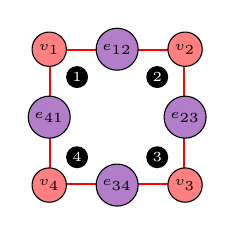
\begin{tikzpicture}
        \node[name=s, regular polygon, regular polygon sides = 4, inner sep = 0.6cm, draw, red, thick] at (0, 0) {};

        \node[draw, circle, fill=red!50!white, inner sep = 1.5pt, text=black] at (s.corner 2) {\tiny{$v_1$}};
        \node[draw, circle, fill=black, inner sep = 1pt, text=white] at ($(s.corner 2) + (315:0.5)$) {\tiny{$1$}};
        \foreach \anchor/\placement/\n/\label in
        {corner 1/below/1/2, corner 3/right/3/4, corner 4/above/4/3}
        {
        \node[draw, circle, fill=red!50!white, inner sep = 1.5pt, text=black] at (s.\anchor) {\tiny{$v_{\label}$}};
        \node[draw, circle, fill=black, inner sep = 1pt, text=white] at ($(s.\anchor) + (135 + \n*90:0.5)$) {\tiny{$\label$}};
        }
        \foreach \anchor/\placement/\n/\label in
        {side 1/below/1/12, side 2/below/2/41, side 3/right/3/34, side 4/above/4/23}
        {
        \node[draw, circle, fill=red!30!white!70!blue, inner sep = 1.5pt, text=black] at (s.\anchor) {\tiny{$e_{\label}$}};
        }
    \end{tikzpicture}
    }
    \label{fig:warmup-labels}
\end{equation}
The ten independent stabilizer generators define a codespace with two logical qubits: 


\begin{equation}
    \cC = \text{span} \{ \ket{\bar{\psi}} \otimes \ket{+}^{\otimes 4}_\vertexV \otimes \ket{0}^{\otimes 4}_\edgeE \} \quad \ket{\bar{\psi}} = \ket{\bar{00}}_{422}, \ket{\bar{01}}_{422},  \ket{\bar{10}}_{422},  \ket{\bar{11}}_{422}
\end{equation}
The code's transversal gate is the alternating phase-gate pattern: 
\begin{equation}
    \T = \Sg_1 \Sg^\dagger_2 \Sg_3 \Sg^\dagger_4
\end{equation}
We consider the logical basis $$\bar{X}_1 = X_1 X_2, \quad \bar{Z}_1 = Z_1 Z_4, $$ $$\bar{X}_2 = X_1 X_4, \quad \bar{Z}_2 = Z_1 Z_2$$
The action of the transversal gate is:
\begin{equation}
\begin{aligned}
    \T \bar{X}_1 \T^\dagger &= (\Sg_1 X_1 \Sg_1^\dagger)( \Sg_2^\dagger X_2 \Sg_2) = -Y_1 Y_2 = X_1 X_2 (Z_1 Z_2) = \bar{X}_1 \bar{Z}_2 \\
    \T \bar{X}_2 \T^\dagger &= (\Sg_1 X_1 \Sg_1^\dagger) (\Sg_4^\dagger X_4 \Sg_4) = -Y_1 Y_4 = X_1 X_4 (Z_1 Z_4) = \bar{X}_2 \bar{Z}_1 \\
\end{aligned}
\end{equation} Thus, this transversal gate yields a logical $CZ$.

While the full transversal circuit $\T$ squares to the identity (up to a stabilizer), in our current presentation, the local action on each vertex set is order four. We can multiply the transversal circuit by the $S_X$ stabilizer to obtain: 
\begin{equation}
    \T=\prod_{v = 1}^4W_v=\CZbar,\qquad
    W_1=W_3=e^{-i\pi/4}XS,\qquad W_2=W_4=e^{+i\pi/4}XS^\dagger ,
    \label{eq:warmup-T}
\end{equation}
Now the action of the transversal gate on each vertex set, given by $W_i$, squares to the identity. Note we have added some additional phases to ensure that the final gauged code stabilizers admit $+1$ eigenspaces.


The gauging circuit consists of three layers (Definition~\ref{def:gauging-circuit}): (1) the symmetry
enrichment (S.E.), which entangles each ancilla with its vertex set by
$C_{v_i}(W_i)$, (2) the cluster entangler (C.E.), and (3) the measurement of the
vertex ancillas in the $X$ basis, which implements the projective measurement of the transversal gate.

The ancilla stabilizer $X_{v_1}$ is pushed through the circuit as follows:


\begin{equation}
\raisebox{-55pt}{
    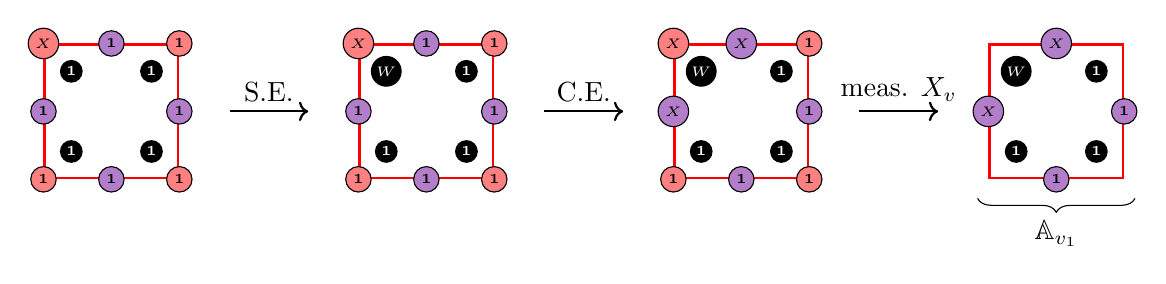
\begin{tikzpicture}
        \node[name=s, regular polygon, regular polygon sides = 4, inner sep = 0.6cm, draw, red, thick] at (0, 0) {};

        \node[draw, circle, fill=red!50!white, inner sep = 1.5pt, text=black] at (s.corner 2) {\tiny{$X$}};
        \node[draw, circle, fill=black, inner sep = 1pt, text=white] at ($(s.corner 2) + (315:0.5)$) {\tiny{$\id$}};
        \foreach \anchor/\placement/\n in
        {corner 1/below/1, corner 3/right/3, corner 4/above/4}
        {
        \node[draw, circle, fill=red!50!white, inner sep = 1.5pt, text=black] at (s.\anchor) {\tiny{$\id$}};
        \node[draw, circle, fill=black, inner sep = 1pt, text=white] at ($(s.\anchor) + (135 + \n*90:0.5)$) {\tiny{$\id$}};
        }
        \foreach \anchor/\placement/\n in
        {side 1/below/1, side 2/below/2, side 3/right/3, side 4/above/4}
        {
        \node[draw, circle, fill=red!30!white!70!blue, inner sep = 1.5pt, text=black] at (s.\anchor) {\tiny{$\id$}};
        }

        \draw[->, thick] (1.5, 0) -- (2.5, 0) node [pos = 0.5, above] {S.E.};

        \node[name=s, regular polygon, regular polygon sides = 4, inner sep = 0.6cm, draw, red, thick] at (4, 0) {};

        \node[draw, circle, fill=red!50!white, inner sep = 1.5pt, text=black] at (s.corner 2) {\tiny{$X$}};
        \node[draw, circle, fill=black, inner sep = 1pt, text=white] at ($(s.corner 2) + (315:0.5)$) {\tiny{$W$}};
        \foreach \anchor/\placement/\n in
        {corner 1/below/1, corner 3/right/3, corner 4/above/4}
        {
        \node[draw, circle, fill=red!50!white, inner sep = 1.5pt, text=black] at (s.\anchor) {\tiny{$\id$}};
        \node[draw, circle, fill=black, inner sep = 1pt, text=white] at ($(s.\anchor) + (135 + \n*90:0.5)$) {\tiny{$\id$}};
        }
        \foreach \anchor/\placement/\n in
        {side 1/below/1, side 2/below/2, side 3/right/3, side 4/above/4}
        {
        \node[draw, circle, fill=red!30!white!70!blue, inner sep = 1.5pt, text=black] at (s.\anchor) {\tiny{$\id$}};
        }
        \draw[->, thick] (5.5, 0) -- (6.5, 0) node [pos = 0.5, above] {C.E.};

        \node[name=s, regular polygon, regular polygon sides = 4, inner sep = 0.6cm, draw, red, thick] at (8, 0) {};

        \node[draw, circle, fill=red!50!white, inner sep = 1.5pt, text=black] at (s.corner 2) {\tiny{$X$}};
        \node[draw, circle, fill=black, inner sep = 1pt, text=white] at ($(s.corner 2) + (315:0.5)$) {\tiny{$W$}};
        \foreach \anchor/\placement/\n in
        {corner 1/below/1, corner 3/right/3, corner 4/above/4}
        {
        \node[draw, circle, fill=red!50!white, inner sep = 1.5pt, text=black] at (s.\anchor) {\tiny{$\id$}};
        \node[draw, circle, fill=black, inner sep = 1pt, text=white] at ($(s.\anchor) + (135 + \n*90:0.5)$) {\tiny{$\id$}};
        }
        \foreach \anchor/\placement/\n in
        {side 3/right/3, side 4/above/4}
        {
        \node[draw, circle, fill=red!30!white!70!blue, inner sep = 1.5pt, text=black] at (s.\anchor) {\tiny{$\id$}};
        }
        \foreach \anchor/\placement/\n in
        {side 1/below/1, side 2/below/2}
        {
        \node[draw, circle, fill=red!30!white!70!blue, inner sep = 1.5pt, text=black] at (s.\anchor) {\tiny{$X$}};
        }
         
        
        \draw[->, thick] (9.5, 0) -- (10.5, 0) node [pos = 0.5, above] {meas. $X_v$};

        \node[name=s, regular polygon, regular polygon sides = 4, inner sep = 0.6cm, draw, red, thick] at (12, 0) {};
        
        \node[draw, circle, fill=black, inner sep = 1pt, text=white] at ($(s.corner 2) + (315:0.5)$) {\tiny{$W$}};
        \foreach \anchor/\placement/\n in
        {corner 1/below/1, corner 3/right/3, corner 4/above/4}
        {
        
        \node[draw, circle, fill=black, inner sep = 1pt, text=white] at ($(s.\anchor) + (135 + \n*90:0.5)$) {\tiny{$\id$}};
        }
        \foreach \anchor/\placement/\n in
        {side 3/right/3, side 4/above/4}
        {
        \node[draw, circle, fill=red!30!white!70!blue, inner sep = 1.5pt, text=black] at (s.\anchor) {\tiny{$\id$}};
        }
        \foreach \anchor/\placement/\n in
        {side 1/below/1, side 2/below/2}
        {
        \node[draw, circle, fill=red!30!white!70!blue, inner sep = 1.5pt, text=black] at (s.\anchor) {\tiny{$X$}};
        }

        \draw [decorate,decoration={brace,amplitude=5pt,mirror,raise=4ex}] (11,-0.5) -- (13,-0.5) node[midway,yshift=-3em]{$\mathbb{A}_{v_1}$};
    \end{tikzpicture}
}
    \label{eq:warmup-flow}
\end{equation}
The gauging graph and vertex ancilla are drawn in red, the edge ancilla in purple, and the original $[[4, 2, 2]]$ degrees of freedom in black. The final step of Eq. \ref{eq:warmup-flow} yields the vertex checks $\mathbb{A}_{v}=W_vX_eX_{e'}$ ($e,e'$ the two loop
edges at $v$), with $\prod_v\mathbb{A}_v=\CZbar$.
Measuring these ancillas thus measures the logical.

Likewise, the initial edge stabilizers $Z_e$
become the cluster checks $L_e=Z_vZ_eZ_{v'}$.
The vertex measurement destroys
them individually, but their product around the loop formed by the gauging graph survives as the flux check
$\bp=\prod_{e \in \edgeE}Z_e=\prod_e L_e$.
\begin{equation}
\raisebox{-32pt}{
    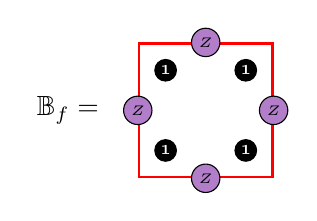
\begin{tikzpicture}
        \node at (0, 0) {$\bp = $};
        \node[name=s, regular polygon, regular polygon sides = 4, inner sep = 0.6cm, draw, red, thick] at (1.75, 0) {};

        \node[draw, circle, fill=black, inner sep = 1pt, text=white] at ($(s.corner 2) + (315:0.5)$) {\tiny{$\id$}};
        \foreach \anchor/\placement/\n in
        {corner 1/below/1, corner 3/right/3, corner 4/above/4}
        {
        \node[draw, circle, fill=black, inner sep = 1pt, text=white] at ($(s.\anchor) + (135 + \n*90:0.5)$) {\tiny{$\id$}};
        }
        \foreach \anchor/\placement/\n in
        {side 1/below/1, side 2/below/2, side 3/right/3, side 4/above/4}
        {
        \node[draw, circle, fill=red!30!white!70!blue, inner sep = 1.5pt, text=black] at (s.\anchor) {\tiny{$Z$}};
        }
        
    \end{tikzpicture}
}
\end{equation}

The matter stabilizers $S_Z,S_X$ do not commute with the $C_{v}(W_v)$ gates involved in the symmetry enrichment step, so their support is expanded onto the vertex qubits. The conjugation of a Pauli operator $P$ with each controlled-$W$ or controlled-$W^\dagger$ gate is as follows:
\begin{equation}
    C_v(W_v)\,P\,C_v(W_v)^\dagger = P\cdot C_v(W_vPW_vP)
\end{equation}
In this example, we use the following commutators:
\begin{equation}
\begin{aligned}
    W_{v_i}Z_iW_{v_i}Z_i=-\id, &\quad i = 1, 2, 3, 4 \\
    W_{v_{i}}X_{i}W_{v_{i}}X_i=-iZ_i, &\quad i = 1, 3 \\
    W_{v_{i}}X_{i}W_{v_{i}}X_i=+iZ_i, &\quad i = 2, 4
\end{aligned}
\label{eq:warmup-remnants}
\end{equation}
The first $Z$-type commutator is simple, and its control evaluates to $C_v(-\id)=Z_v$. The $X$ check instead picks up controlled-$Z$ remnants
dressed by phase gates, $C_v(\mp iZ)=\Sg_v^{\mp1}\,C_v(Z_{q_v})$. These phase gates arise from the local phases in the group commutators, and 
tracking them locally is a subtlety of the gauging procedure. Nevertheless, globally they cancel, $(-i)(+i)(-i)(+i)\,ZZZZ=S_Z$, yielding one of the code's stabilizers.


The symmetry-enrichment (S.E.) layer sends $S_Z\mapsto S_Z\prod_vZ_v$, since each
decoration is the control $C_v(-\id)=Z_v$. Enforcing the stabilizer constraint $L_e=+1$ pairwise
yields the additional constraints $Z_{v_1}Z_{v_2}=Z_{e_{12}}$ and $Z_{v_3}Z_{v_4}=Z_{e_{34}}$.
These allow us to move the vertex support onto the edges to yield $\gaugedS_Z=ZZZZ\cdot Z_{e_{12}}Z_{e_{34}}$.
In other words, our derivation is only concerned with ensuring commutation relations within the $+1$ eigenspace, 
and the form and algebraic relations of the gauged stabilizers can change outside of that space. Pictorially, the transformation of the $S_Z$ stabilizer under the gauging circuit is as follows:
\begin{equation}
\raisebox{-55pt}{
    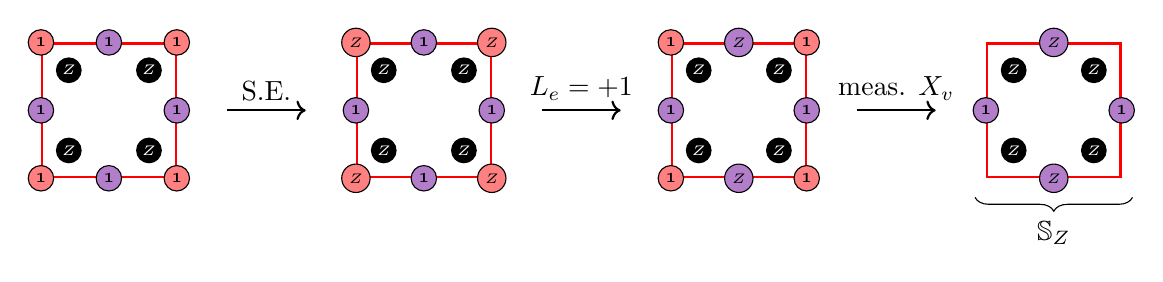
\begin{tikzpicture}
        \node[name=s, regular polygon, regular polygon sides = 4, inner sep = 0.6cm, draw, red, thick] at (0, 0) {};

        \foreach \anchor/\placement/\n in
        {corner 1/below/1, corner 2/right/2, corner 3/right/3, corner 4/above/4}
        {
        \node[draw, circle, fill=red!50!white, inner sep = 1.5pt, text=black] at (s.\anchor) {\tiny{$\id$}};
        \node[draw, circle, fill=black, inner sep = 1pt, text=white] at ($(s.\anchor) + (135 + \n*90:0.5)$) {\tiny{$Z$}};
        }
        
        \foreach \anchor/\placement/\n in
        {side 1/below/1, side 2/below/2, side 3/right/3, side 4/above/4}
        {
        \node[draw, circle, fill=red!30!white!70!blue, inner sep = 1.5pt, text=black] at (s.\anchor) {\tiny{$\id$}};
        }

        \draw[->, thick] (1.5, 0) -- (2.5, 0) node [pos = 0.5, above] {S.E.};

        \node[name=s, regular polygon, regular polygon sides = 4, inner sep = 0.6cm, draw, red, thick] at (4, 0) {};

        \foreach \anchor/\placement/\n in
        {corner 1/below/1, corner 2/right/2, corner 3/right/3, corner 4/above/4}
        {
        \node[draw, circle, fill=red!50!white, inner sep = 1.5pt, text=black] at (s.\anchor) {\tiny{$Z$}};
        \node[draw, circle, fill=black, inner sep = 1pt, text=white] at ($(s.\anchor) + (135 + \n*90:0.5)$) {\tiny{$Z$}};
        }
        \foreach \anchor/\placement/\n in
        {side 1/below/1, side 2/below/2, side 3/right/3, side 4/above/4}
        {
        \node[draw, circle, fill=red!30!white!70!blue, inner sep = 1.5pt, text=black] at (s.\anchor) {\tiny{$\id$}};
        }
        \draw[->, thick] (5.5, 0) -- (6.5, 0) node [pos = 0.5, above] {$L_e = +1$};

        \node[name=s, regular polygon, regular polygon sides = 4, inner sep = 0.6cm, draw, red, thick] at (8, 0) {};

        \foreach \anchor/\placement/\n in
        {corner 1/below/1, corner 2/right/2, corner 3/right/3, corner 4/above/4}
        {
        \node[draw, circle, fill=red!50!white, inner sep = 1.5pt, text=black] at (s.\anchor) {\tiny{$\id$}};
        \node[draw, circle, fill=black, inner sep = 1pt, text=white] at ($(s.\anchor) + (135 + \n*90:0.5)$) {\tiny{$Z$}};
        }
        \foreach \anchor/\placement/\n in
        {side 1/below/1, side 3/right/3}
        {
        \node[draw, circle, fill=red!30!white!70!blue, inner sep = 1.5pt, text=black] at (s.\anchor) {\tiny{$Z$}};
        }
        \foreach \anchor/\placement/\n in
        {side 2/below/2, side 4/right/4}
        {
        \node[draw, circle, fill=red!30!white!70!blue, inner sep = 1.5pt, text=black] at (s.\anchor) {\tiny{$\id$}};
        }
         
        
        \draw[->, thick] (9.5, 0) -- (10.5, 0) node [pos = 0.5, above] {meas. $X_v$};

        \node[name=s, regular polygon, regular polygon sides = 4, inner sep = 0.6cm, draw, red, thick] at (12, 0) {};

        \foreach \anchor/\placement/\n in
        {corner 1/below/1, corner 2/right/2, corner 3/right/3, corner 4/above/4}
        {
        \node[draw, circle, fill=black, inner sep = 1pt, text=white] at ($(s.\anchor) + (135 + \n*90:0.5)$) {\tiny{$Z$}};
        }
        \foreach \anchor/\placement/\n in
        {side 1/below/1, side 3/right/3}
        {
        \node[draw, circle, fill=red!30!white!70!blue, inner sep = 1.5pt, text=black] at (s.\anchor) {\tiny{$Z$}};
        }
        \foreach \anchor/\placement/\n in
        {side 2/below/2, side 4/right/4}
        {
        \node[draw, circle, fill=red!30!white!70!blue, inner sep = 1.5pt, text=black] at (s.\anchor) {\tiny{$\id$}};
        }
        \draw [decorate,decoration={brace,amplitude=5pt,mirror,raise=4ex}] (11,-0.5) -- (13,-0.5) node[midway,yshift=-3em]{$\gaugedS_{Z}$};
    \end{tikzpicture}
}
    \label{eq:warmup-decorated-Z}
\end{equation}


The transformation of the $S_X$ stabilizers under the gauging circuit is a little more complicated. After the symmetry enrichment step, we find:
\begin{equation}
\raisebox{-32pt}{
    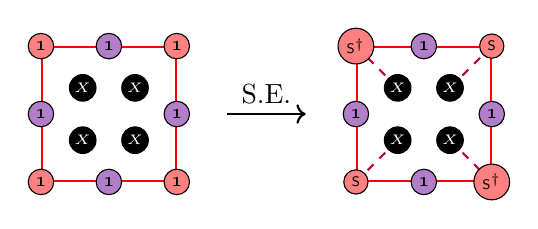
\begin{tikzpicture}
        \node[name=s, regular polygon, regular polygon sides = 4, inner sep = 0.6cm, draw, red, thick] at (0, 0) {};

        \foreach \anchor/\placement/\n in
        {corner 1/below/1, corner 2/right/2, corner 3/right/3, corner 4/above/4}
        {
        \node[draw, circle, fill=red!50!white, inner sep = 1.5pt, text=black] at (s.\anchor) {\tiny{$\id$}};
        \node[draw, circle, fill=black, inner sep = 1pt, text=white] at ($(s.\anchor) + (135 + \n*90:0.75)$) {\tiny{$X$}};
        }
        
        \foreach \anchor/\placement/\n in
        {side 1/below/1, side 2/below/2, side 3/right/3, side 4/above/4}
        {
        \node[draw, circle, fill=red!30!white!70!blue, inner sep = 1.5pt, text=black] at (s.\anchor) {\tiny{$\id$}};
        }

        \draw[->, thick] (1.5, 0) -- (2.5, 0) node [pos = 0.5, above] {S.E.};

        \node[name=s, regular polygon, regular polygon sides = 4, inner sep = 0.6cm, draw, red, thick] at (4, 0) {};

        \foreach \anchor/\text/\n in
        {corner 1/\Sg/1/, corner 2/\Sg^\dagger/2, corner 3/\Sg/3, corner 4/\Sg^\dagger/4}
        {
        \draw[thick, purple, dashed] (s.\anchor) to ($(s.\anchor) + (135 + \n*90:0.75)$); 
        \node[draw, circle, fill=red!50!white, inner sep = 1.5pt, text=black] at (s.\anchor) {\tiny{$\text$}};
        \node[draw, circle, fill=black, inner sep = 1pt, text=white] at ($(s.\anchor) + (135 + \n*90:0.75)$) {\tiny{$X$}};
        }
        \foreach \anchor/\placement/\n in
        {side 1/below/1, side 2/below/2, side 3/right/3, side 4/above/4}
        {
        \node[draw, circle, fill=red!30!white!70!blue, inner sep = 1.5pt, text=black] at (s.\anchor) {\tiny{$\id$}};
        }
    \end{tikzpicture}
    }
    \label{eq:warmup-decorated-X}
\end{equation}
Here the dashed purple line indicates a physical $CZ$. The phase gates and controls that now sit on the vertex ancilla must be moved off before those degrees of freedom are measured in the $X$ basis. After the cluster entangler step, we can use the fact our code subspace now has the constraint $L_e = +1$ to deform the controlled gates away from the vertex ancilla. Indeed, for $U^2=(-1)^m\id$, we have
\begin{equation}
    C_v(U)\;\xrightarrow{\;L_e=+1\;}\;C_e(U)\,C_{v'}(U)\,CZ^{\,m}_{e,v'} .
    \label{eq:warmup-move}
\end{equation}
where the edge $e$ connects vertices $v, v'$. In our case, we can write $\Sg CZ = C(iZ)$, so we have $m = 1$. Thus, for any vertex set, we can replace $C_{v_i}(\pm i Z)_i$ with 
\begin{equation}
    C_{v_i}(\pm i Z)_i \to C_{v_{j}} (\pm i Z)_i C_{e_{i, j}} (\pm i Z)_i  CZ_{e_{ij}, v_{j}}, \quad j = i \pm 1 ~(\text{mod } 4) 
\end{equation}
Starting from vertex $v_4$ and iterating the application of Eq. \eqref{eq:warmup-move} clockwise to the ``root'' vertex $v_1$ we find:
\begin{equation}
    \prod_{i = 1}^4 C_{v_i}(\pm i Z)_i \to C_{e_{34}}(iZ_4)\cdot C_{e_{23}}(Z_3Z_4Z_{e_{34}})\cdot
C_{e_{12}}(iZ_2Z_3Z_4Z_{e_{34}})\cdot C_{v_1}(\gaugedS_Z)
\end{equation}
The last term, $C_{v_1}(\gaugedS_Z)$, is a ``leftover'' piece we can discard because it acts trivially on the codespace where $\gaugedS_Z=+1$. Note that some of these $CZ$ gates can be further simplified; for instance, we have the combination 
$$C_4 (Z_{e_{12}} Z_{e_{23}} Z_{e_{34}} ) \xrightarrow{\bp = +1} C_4 (Z_{e_{41}})$$
Expanding (and performing the above simplification) the gauged $S_X$ stabilizer in terms of elementary gates yields
\begin{equation}
    \raisebox{-47pt}{
    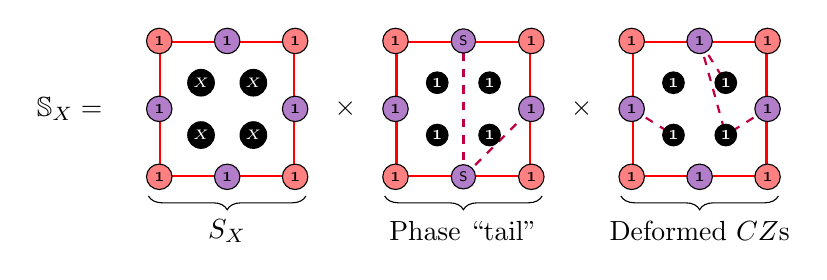
\begin{tikzpicture}

        \node at (-2, 0) {$\gaugedS_X = $};
        \node[name=s, regular polygon, regular polygon sides = 4, inner sep = 0.6cm, draw, red, thick] at (0, 0) {};

        \foreach \anchor/\n in
        {corner 1/1/, corner 2/2, corner 3/3, corner 4/4}
        {
        \node[draw, circle, fill=red!50!white, inner sep = 1.5pt, text=black] at (s.\anchor) {\tiny{$\id$}};
        \node[draw, circle, fill=black, inner sep = 1pt, text=white] at ($(s.\anchor) + (135 + \n*90:0.75)$) {\tiny{$X$}};
        }
        \foreach \anchor/\placement/\n in
        {side 1/below/1, side 2/below/2, side 3/right/3, side 4/above/4}
        {
        \node[draw, circle, fill=red!30!white!70!blue, inner sep = 1.5pt, text=black] at (s.\anchor) {\tiny{$\id$}};
        }

        \draw [decorate,decoration={brace,amplitude=5pt,mirror,raise=4ex}] (-1,-0.5) -- (1,-0.5) node[midway,yshift=-3em]{$S_X$};


        \node at (1.5, 0) {$\times$};

        
        \node[name=s, regular polygon, regular polygon sides = 4, inner sep = 0.6cm, draw, red, thick] at (3, 0) {};
        
        \draw[thick, purple, dashed] (s.side 3) to (s.side 4);
        \draw[thick, purple, dashed] (s.side 3) to (s.side 1);
        
        \foreach \anchor/\n in
        {corner 1/1/, corner 2/2, corner 3/3, corner 4/4}
        {
        \node[draw, circle, fill=red!50!white, inner sep = 1.5pt, text=black] at (s.\anchor) {\tiny{$\id$}};
        \node[draw, circle, fill=black, inner sep = 1pt, text=white] at ($(s.\anchor) + (135 + \n*90:0.75)$) {\tiny{$\id$}};
        }
        \foreach \anchor/\placement/\n/\text in
        {side 1/below/1/\Sg, side 2/below/2/\id, side 3/right/3/\Sg, side 4/above/4/\id}
        {
        \node[draw, circle, fill=red!30!white!70!blue, inner sep = 1.5pt, text=black] at (s.\anchor) {\tiny{$\text$}};
        }

        \draw [decorate,decoration={brace,amplitude=5pt,mirror,raise=4ex}] (2,-0.5) -- (4,-0.5) node[midway,yshift=-3em]{Phase ``tail''};


        \node at (4.5, 0) {$\times$};

        
        \node[name=s, regular polygon, regular polygon sides = 4, inner sep = 0.6cm, draw, red, thick] at (6, 0) {};
        
        \draw[thick, purple, dashed] (s.side 1) to ($(s.corner 1) + (135 + 1*90:0.75)$);
        \draw[thick, purple, dashed] (s.side 1) to ($(s.corner 4) + (135 + 4*90:0.75)$);

        \draw[thick, purple, dashed] (s.side 4) to ($(s.corner 4) + (135 + 4*90:0.75)$);

        \draw[thick, purple, dashed] (s.side 2) to ($(s.corner 3) + (135 + 3*90:0.75)$);
        
        \foreach \anchor/\n in
        {corner 1/1/, corner 2/2, corner 3/3, corner 4/4}
        {
        
        \node[draw, circle, fill=red!50!white, inner sep = 1.5pt, text=black] at (s.\anchor) {\tiny{$\id$}};
        \node[draw, circle, fill=black, inner sep = 1pt, text=white] at ($(s.\anchor) + (135 + \n*90:0.75)$) {\tiny{$\id$}};
        }
        \foreach \anchor/\placement/\n/\text in
        {side 1/below/1/\id, side 2/below/2/\id, side 3/right/3/\id, side 4/above/4/\id}
        {
        \node[draw, circle, fill=red!30!white!70!blue, inner sep = 1.5pt, text=black] at (s.\anchor) {\tiny{$\text$}};
        }

        \draw [decorate,decoration={brace,amplitude=5pt,mirror,raise=4ex}] (5,-0.5) -- (7,-0.5) node[midway,yshift=-3em]{Deformed $CZ$s};
        
        
    \end{tikzpicture}
    }
\end{equation}

Every check above squares to one, and any two stabilizers commute, with a single exception: the decorated $X$ check and
the \emph{root} vertex check, whose group commutator,
$\mathbb{A}_{v_1}\,\gaugedS_X\,\mathbb{A}_{v_1}\gaugedS_X=\gaugedS_Z$, nevertheless remains in the stabilizer group.
These two checks therefore commute precisely on the codespace, where $\gaugedS_Z=+1$, and anticommute on the $\gaugedS_Z=-1$ sector. Note that the gauged codespace is \emph{three}-dimensional, the dimension of the $\CZbar=+1$ eigenspace rather than a power of two.

We return to (almost) the original code by measuring the gauge degrees of freedom in the computational basis; this will project out all the decorations we have added to the $[[4, 2, 2]]$ stabilizers, up to an application of some of the $W_{v_i}$. More specifically, since we had $\bp = +1$ prior to measuring out the edge ancillas, we should end up with an even number of $\ket{1}$ outcomes. For instance, suppose we measured $Z_{e_{12}} = Z_{e_{23}} = +1$ and $Z_{e_{34}} = Z_{e_{41}} = -1$. Then the decorated stabilizers become: 
\begin{equation}
    \raisebox{-35pt}{
    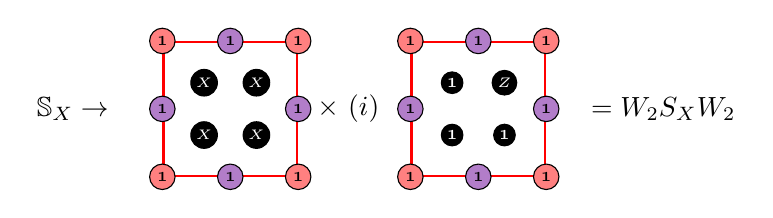
\begin{tikzpicture}

        \node at (-2, 0) {$\gaugedS_X \to $};
        \node[name=s, regular polygon, regular polygon sides = 4, inner sep = 0.6cm, draw, red, thick] at (0, 0) {};

        \foreach \anchor/\n in
        {corner 1/1/, corner 2/2, corner 3/3, corner 4/4}
        {
        \node[draw, circle, fill=red!50!white, inner sep = 1.5pt, text=black] at (s.\anchor) {\tiny{$\id$}};
        \node[draw, circle, fill=black, inner sep = 1pt, text=white] at ($(s.\anchor) + (135 + \n*90:0.75)$) {\tiny{$X$}};
        }
        \foreach \anchor/\placement/\n in
        {side 1/below/1, side 2/below/2, side 3/right/3, side 4/above/4}
        {
        \node[draw, circle, fill=red!30!white!70!blue, inner sep = 1.5pt, text=black] at (s.\anchor) {\tiny{$\id$}};
        }


        \node at (1.5, 0) {$\times ~(i) $};

        
        \node[name=s, regular polygon, regular polygon sides = 4, inner sep = 0.6cm, draw, red, thick] at (3.15, 0) {};
        
        \foreach \anchor/\n/\text in
        {corner 1/1/Z, corner 2/2/\id, corner 3/3/\id, corner 4/4/\id}
        {
        \node[draw, circle, fill=red!50!white, inner sep = 1.5pt, text=black] at (s.\anchor) {\tiny{$\id$}};
        \node[draw, circle, fill=black, inner sep = 1pt, text=white] at ($(s.\anchor) + (135 + \n*90:0.75)$) {\tiny{$\text$}};
        }
        \foreach \anchor/\placement/\n/\text in
        {side 1/below/1/\id, side 2/below/2/\id, side 3/right/3/\id, side 4/above/4/\id}
        {
        \node[draw, circle, fill=red!30!white!70!blue, inner sep = 1.5pt, text=black] at (s.\anchor) {\tiny{$\text$}};
        }


        \node at (5.5, 0) {$ = W_2 S_X W_2$};

        
        
    \end{tikzpicture}
    }
\end{equation}
\begin{equation}
    \gaugedS_Z \to - S_Z = W_2 S_Z W_2
\end{equation}
We obtain $S_X$ and $S_Z$ by applying $W_2$ again. It is straightforward to check for any other set of consistent edge measurement outcomes that the necessary correction is some combination of the $W_i$. 

Meanwhile, only the product $\CZbar = \prod_v \av$ is preserved when we measure out the edge ancilla, ensuring we end up in an eigenstate of $\CZbar$ in the \emph{original} codespace. 

Thus, measuring $\CZbar$ on it can prepare the $\ket{CZ}$ magic
states used in Section~\ref{sec:applications}, if we find the parity of the $\av$ stabilizers is $+1$. If we have an odd number of violated $\av$, we would infer $\CZbar = -1$, and thus prepare the (non-magical) logical state $\ket{11}$ when we return to the original code. In this case, we reset the logical state of the code to $\ket{++}$ and attempt the gauging process again. Only a constant number of tries should be necessary, scaling with the overlap of the initial logical state and the desired magic state.



\subsection{Qubit codes with $\mathbb{Z}_2$ Clifford transversal gates}

We now briefly consider the special case where $p = q = 2$, as this case demonstrates some additional structure that is not seen in the general case. Given that in this case the ancillary degrees of freedom have the same dimensionality as the local degrees of freedom of the code, we write all Pauli operators as $X$ and $Z$.
Take a qubit code $\cC$ with transversal gate $\T$ such that $\T^2 = \id$. It is straightforward to show that the stabilizers of $\cC$ fall into two groups, $\{S\}$ and $\{N\}$, such that 
\begin{equation}
\label{eq:global-z2-commutation}
    \ComGrp{S}{\T} = N_S \in \{N\}, \quad \ComGrp{N}{\T} = \id
\end{equation}
All stabilizers in $\{N\}$ commute with the operator $\T$, and any other stabilizer $S \in \{S\}$ commutes with $\T$ up to an element of $\{N\}$, which we will denote $N_S$.

We will show that the gauged code has stabilizers as given in Theorem \ref{thm:z2-gauged-stabilizers}.



\begin{theorem}[$\mathbb{Z}_2$ Gauged Stabilizers] \label{thm:z2-gauged-stabilizers}
Given a Pauli stabilizer code $\cC$, a transversal gate such that $\T^2 = \id$, a choice of vertex set $\Sigma$, and a gauging graph $\graphG = (\vertexV, \edgeE)$, the gauged code stabilizers have the following generic form:
    \begin{align}
    \gaugedS = \mathfrak{C}_{2}[S] = S \cdot \left ( \prod_{\substack{v \neq v_0 \\ v \in \invvertexset{S}}} \mathsf{S}^{\mu_v}_{p(v, v_0)} \prod_{e \in p(v, v_0)} C_e(N_S)_v \right ), \label{eq:z2-decorated-stabilizers} \\
    N_S = \ComGrp{S}{\T}, \quad i^{\mu_v} (N_S)_v = \ComGrp{S_v}{\T_v}
\end{align} 
\begin{equation}
    \av = \T_v \prod_{e \in \delta v} X_e, \quad \bp = \prod_{e \in \partial_2 f} Z_e, \quad f \text{ is a face of } \graphG
    \label{eq:av-bp-stabilizers}
\end{equation}
The set $\invvertexset{S} \subseteq \vertexV$ includes all vertex sets in the support of the stabilizer $S$, and the map $\partial_2$ takes a face of $\graphG$ to its boundary edges. We have chosen a \emph{root} vertex $v_0$ for every stabilizer of the initial code, and $p(v, v_0) \subseteq \edgeE$ is a path between vertices $v, v_0$ on the gauging graph. Additionally, $$\mathsf{S}_{p(v, v_0)} \equiv \frac{\id + \prod_{e \in p(v, v_0)} Z_e}{2} + i \frac{\id - \prod_{e \in p(v, v_0)}Z_e}{2}.$$
\end{theorem}
\begin{proof}
    See below.
\end{proof}

The ``invariant'' stabilizers $\{N\}$ are useful to define because they will partially control the non-Abelian (non-stabilizer) behavior of the gauged code: $\av$ and $\gaugedS$ stabilizers of the gauged code only commute up to the gauged version of some element of $\{N\}$ (see Corollary \ref{cor:z2-commutation-relations} below). 


\begin{corollary}[Commutation relations of Clifford-decorated stabilizers]
\label{cor:z2-commutation-relations}
The nontrivial commutation relations between the stabilizers in Theorem \ref{thm:z2-gauged-stabilizers} are given by:
\begin{align}
    \ComGrp{\gaugedS}{\mathbb{A}_{v_0}}
    =\mathbb{N}_S,
    \qquad
    \mathbb{N}_S=\mathfrak{C}_2[N_S].
\end{align}
\begin{equation}
    \ComGrp{\gaugedS_i}{\gaugedS_j}
    =\mathbb{B}_{f(i,j)},
\end{equation}
for some cycle $f(i,j)$.  The remaining commutators are trivial on the full Hilbert space:
\begin{equation}
    \ComGrp{\bp}{\av}
    =
    \ComGrp{\bp}{\gaugedS}
    =
    \id.
\end{equation}
\end{corollary}
\begin{proof}
    See Appendix~\ref{app:gauging-procedure-proofs}, Proof~\ref{proof:clifford-decorated-commutation-relations}.
\end{proof}


We will now derive Theorem \ref{thm:z2-gauged-stabilizers}. We assume some choice of gauging graph $\graphG = (\vertexV, \edgeE)$ and some choice of vertex sets $\Sigma: \physq \to \vertexV$. 


\textbf{Symmetry Enrichment:} The first step of the gauging map as defined in Eq. \ref{eq:gauging-circuit} is to apply $\T_v$ to each vertex set, controlled on the corresponding vertex ancilla: this is the ``symmetry enrichment'' step. All stabilizers of the original code $\cC$ will be deformed: 



\begin{equation}
    \begin{aligned}
        S & \xrightarrow{S.E.} S \cdot \prod_{v \in \invvertexset{S}} C_v \ComGrp{S_v}{\T_v}\\
        N_S & \xrightarrow{S.E.} N_S \cdot \prod_{v \in \invvertexset{N_S}} C_v \ComGrp{(N_S)_v}{\T_v}
    \end{aligned}
\end{equation}
Although we defined the commutation relation between the stabilizers and the full transversal gate $\T$ in Eq. \ref{eq:global-z2-commutation}, the commutation relations when restricted to a given vertex set may differ by a phase. In particular, due to the fact we are dealing with Pauli stabilizers, a Clifford operator $\T$, and we know $\ComGrp{S}{\T} = N_S$, it is straightforward to show that
\begin{equation}
    \ComGrp{S_v}{\T_v} = i^{\mu_v} (N_S)_v, \quad \ComGrp{(N_S)_v}{\T_v} = i^{2\mu_v} = (-1)^{\mu_v} 
\end{equation}
for some $\mu_v = 0, 1, 2, 3$. Since for any stabilizer $S$, $\ComGrp{S}{\T}$ must be Hermitian, we must have $i^{\sum_v \mu_v} = 1 \implies \sum_v \mu_v = 0 ~(\text{mod } 4)$, summing over $v \in \invvertexset{S}$. 

The vertex ancilla are initialized in the $\ket{+}$ state, and so under the symmetry enrichment circuit their stabilizers are deformed as well:
\begin{equation}
    X_v \xrightarrow{S.E} X_v \T_v
\end{equation}

\textbf{Cluster Entangler:} The next step of the gauging map is to apply the graph cluster entangler between the vertex ancilla and the edge ancilla, which we initialize in the $\ket{0}$ state. The graph cluster entangler is defined as: 
\begin{equation}
    \prod_{v \in \vertexV} \prod_{e \in \delta v} C_v X_e
\end{equation}
Only the vertex stabilizers and the edge ancilla stabilizers are impacted: 
\begin{equation}
    X_v \T_v \xrightarrow{C.E.} X_v \T_v \prod_{e \in \delta v} X_e
\end{equation}
\begin{equation}
    Z_e \to L_e = Z_{v} Z_{e} Z_{v'}, \quad \partial e = \{v, v'\}
\end{equation}
Recall that $\delta: \vertexV \to \edgeE$ and $\partial: \edgeE \to \vertexV$ are the co-boundary and boundary maps of $\graphG$. 

\textbf{Measuring out vertices:} For the final step, we project the vertex ancilla back to the $\ket{+}$ state. The deformed vertex stabilizers become the $\av$ stabilizers:
\begin{equation}
    X_v \T_v \prod_{e \in \delta v} X_e \xrightarrow{\dyad{+}} \av = \T_v \prod_{e \in \delta v} X_e
\end{equation}
Let $p \subseteq \edgeE$ be a collection of edges forming a closed path. This defines the stabilizer $\bp$, which commutes with the projector $\dyad{+}$, although individual $L_e$ stabilizers do not.
\begin{equation}
    \prod_{e \in p, \partial p = 0} L_e = \prod_{e \in p} Z_e \xrightarrow{\dyad{+}} \bp 
\end{equation}
To find the surviving deformed stabilizers of the original code after the projection, we need to push the support of the control gates away from the vertex ancilla. For the invariant stabilizers $N_S$, we can use the $L_e$ stabilizers directly to push support away from the vertex ancilla:
\begin{equation}
\begin{aligned}
    N_S \cdot \prod_{v \in \invvertexset{N_S}} C_v \ComGrp{(N_S)_v}{\T_v}  &= N_S \cdot \prod_{v \in \invvertexset{N_S}} Z_v^{\mu_v} \\
    &\xrightarrow{L_e = +1} \mathbb{N}_S \equiv N_S \prod_{v \in \invvertexset{N_S} / \{v_0\}} \prod_{e \in p(v, v_0)} Z_e^{\mu_v}
\end{aligned}
\end{equation}
Here, $v_0$ is some ``root'' vertex we have chosen by convention, and $p(v, v_0) \subseteq \edgeE$ is a path connecting vertices $v, v_0$ on the gauging graph $\graphG$ ($\partial p(v, v_0) = \{v, v_0\}$). There is no longer any support on the vertex ancilla, and so under the projection, this stabilizer remains unchanged: $\mathbb{N}_S \xrightarrow{\dyad{+}} \mathbb{N}_S$.


For the other stabilizers $\{S\}$, we use the following identities, which are valid on the subspace where $L_e = +1$:



\begin{equation}
    C_v U \xrightarrow{L_e = +1} C_{u} U \prod_{e \in p(v, u)} C_e U \equiv C_{u} U \cdot C_{p(v, u)} U, \quad U = U^\dagger
    \label{eq:control-gate-pushing}
\end{equation}
\begin{equation}
    \mathsf{S}^{\mu_v}_{v} \mathsf{S}^{-{\mu_v}}_{u} \xrightarrow{L_e = +1} \mathsf{S}^{\mu_v}_{p(v, u)} \cdot \prod_{e \in p(v, u)} (C_uZ_{e})^{\mu_v}, \quad \mathsf{S}_{p(v, u)} \equiv \frac{1 + \prod_{e \in p(v, u)} Z_e}{2} + i \frac{1 - \prod_{e \in p(v, u)}Z_e}{2}
    \label{eq:S-vertex-edge-identity}
\end{equation}
Applying these to the deformed $S$ stabilizer after the cluster entangler step yields:
\begin{equation}
\begin{aligned}
    S \cdot \prod_{v \in \invvertexset{S}} C_v \ComGrp{S_v}{\T_v} &= S \cdot \prod_{v \in \invvertexset{S}} \Sg^{\mu_v}_{v} C_v (N_S)_v \\ 
    \xrightarrow{L_e = +1} S \cdot &C_{v_0} \left ( N_S \prod_{v \neq v_0} \prod_{e \in p(v, v_0)} Z_e^{\mu_v}  \right ) \cdot \left ( \prod_{v \neq v_0} \mathsf{S}^{\mu_v}_{p(v, v_0)} \prod_{e \in p(v, v_0)} C_e (N_S)_v \right ) \\
    &= S \cdot C_{v_0} \mathbb{N}_S \cdot \left ( \prod_{v \neq v_0} \mathsf{S}^{\mu_v}_{p(v, v_0)} \prod_{e \in p(v, v_0)} C_e(N_S)_v \right )
\end{aligned}
\end{equation}
Here, $v \neq v_0$ is understood to mean the set $\invvertexset{S} / \{v_0\}$. There is still support on the root vertex ancilla, $v_0$. However, it is in the form of a controlled $\mathbb{N}_S$ stabilizer. In the gauged code's codespace, $\mathbb{N}_S = +1$, and so this controlled-gate acts trivially. Thus, we can remove it to obtain a deformed stabilizer $\gaugedS$ that commutes with the projection $\dyad{+}$:
\begin{equation}
    S \cdot C_{v_0} \mathbb{N}_S \cdot \left ( \prod_{v \neq v_0} \mathsf{S}^{\mu_v}_{p(v, v_0)} \prod_{e \in p(v, v_0)} C_e(N_S)_v \right ) \xrightarrow{\mathbb{N}_S = +1} \gaugedS \equiv S \cdot \left ( \prod_{v \neq v_0} \mathsf{S}^{\mu_v}_{p(v, v_0)} \prod_{e \in p(v, v_0)} C_e(N_S)_v \right ) 
    \label{eq:z2-decorated-stabilizers-final}
\end{equation}
Note that this expression holds for $\mathbb{N}_S$ stabilizers as well. In this case, $N_{N_S} = \id$, killing the control gates, while $\mu_v = 0, 2$ for all vertex sets, turning the phase gates $\Sg$ into products of Pauli $Z$. This completes the proof of Theorem \ref{thm:z2-gauged-stabilizers}: we have derived the stated expressions for the gauged code stabilizers. 




\begin{remark}[Measuring non-Hermitian stabilizers]\label{rem:measurement-circuit}
    From Eqs. \ref{eq:z2-decorated-stabilizers}~-~\ref{eq:av-bp-stabilizers} we see that the gauged stabilizers are always unitary, though not Hermitian in general. 
    It is always possible to ``measure'' a non-Hermitian but unitary operator by using an ancilla qudit to project onto one of its eigenspaces and measuring the ancilla to learn onto which eigenspace the state was projected.
    This is achievable through a generalized quantum phase estimation circuit~\cite{kitaev1995quantummeasurementsabelianstabilizer}.
\end{remark}

\subsection{Structure of generic gauged codes}

In the general case, where we have a qudit code and a $\mathbb{Z}_p$ symmetry, we cannot draw on the structure we took advantage of in the previous section. The resulting gauged stabilizers are not in general unitary, but we can still write down operators that define the gauged codespace.

\begin{theorem}[Generic Gauged Stabilizers]
    Consider a qudit code $\cC = \langle S \rangle$ with transversal gate $\T$ such that $\T^p = \id$. Assume some $\Sigma, \graphG = (\vertexV, \edgeE)$. We assign an ancillary qu(p)it to each vertex $v \in \vertexV$ and each edge $e \in \edgeE$. The vertices are initialized in the $\Xp = +1$ eigenstate while the edges are initialized in the $\Zp = +1$ computational basis state. 

    Define the symmetrized stabilizers 
    \begin{equation}
        \sym = \frac{1}{p} \sum_{a = 0}^{p-1} \T^a S (\T^a)^\dagger
    \end{equation}

    Then the gauged code $\cC'$ has stabilizers:
    \begin{equation}
        \av = \T_v \prod_{e \in \delta v} \Xp_e^{\eta_v(e)}, \quad \bp = \prod_{e \in p} \Zp^{\eta_p(e)}_e, \quad \bar{\mathbb{S}} = \Circo[\sym]
    \end{equation}
    \begin{equation}
        \Circo[\sym] = \sum_{\mathbf{a'}}  \prod_{v \neq v_0} \prod_{e \in p(v, v_0)} \dyad{\eta_p(e) a_v'}_e \otimes \T^{\mathbf{a'}}_{v \neq v_0} \sym (\T^{\mathbf{a'}}_{v \neq v_0})^\dagger 
    \end{equation}
    \label{thm:generic-gauged-stabilizers}
\end{theorem}
\begin{proof}
    The derivation of the $\av$ and $\bp$ stabilizers is much the same as the $\mathbb{Z}_2$ case.
\begin{equation}
    \av =  \T_v \prod_{e \in \delta v} \Xp_e^{\eta_v(e)}, \quad 
    \bp = \prod_{e \in \partial p} \Zp^{\eta_p(e)}_e 
\end{equation} where $\eta_v(e) = \pm 1$ captures whether an edge $e$ is going into or out of a given vertex $v$, while $\eta_p(e) = \pm 1$ denotes whether the edge $e$ is aligned or anti-aligned with the orientation of the path (here, a cycle) $p$. 

The bare stabilizers of the code $\cC$ can no longer be separated into invariant stabilizers $\{N\}$ and variant stabilizers $\{S\}$ under the action of $\T$. Instead, we consider ``symmetrized'' stabilizers:
\begin{align}
    \sym = \frac{1}{p} \sum_{a = 0}^{p-1} \T^a S (\T^a)^\dagger
\end{align} Immediately, we see that $\sym$ is invariant under the action of $\T$:
\begin{equation}
    \T^b \sym (\T^b)^\dagger = \sym, \quad b = 0, \dots, p-1
\end{equation} 
Under the symmetry enrichment step, we have: 
\begin{align}
    \sym &\xrightarrow{\textrm{S.E.}} \sum_{\mathbf{a}} \dyad{\mathbf{a}}_{\invvertexset{S}} \otimes \T^{\mathbf{a}} \sym (\T^{\mathbf{a}})^\dagger, \quad \mathbf{a} \in \mathbf{F}_{p}^{|\invvertexset{S}|}, \quad
    \T^{\mathbf{a}} \equiv \prod_{v \in \invvertexset{S}} \T^{a_v}_v
\end{align}
Note that this is not a trivial deformation, as $\sym$ is not necessarily invariant under the local action $\T_v$. The deformed $\sym$ is left unchanged by the cluster entangler, although we should remember that now the stabilizers $L_e =(\Zp_{v}^\dagger \Zp_e \Zp_{v'})^{\eta_v(e)}$ have been introduced.

Before we project out the vertex ancilla in the $\dyad{+}$ basis, we need to remove any support from the vertex ancilla that anti-commutes with this projection. Pick a root vertex $v_0 \in \invvertexset{S}$. We will re-index the sum over $\mathbf{a}$ in terms of its component $a_0$ on the vertex $v_0$:



\begin{align}
    \sum_{\mathbf{a}} \dyad{\mathbf{a}}_{\invvertexset{S}} &= \sum_{\mathbf{a'}} \sum_{a_0 = 0}^{p-1} \dyad{a_0}_{v_0} \otimes \dyad{\mathbf{a'}}_{v\neq v_0}, \quad \mathbf{a'} \in \mathbf{F}_p^{|\invvertexset{S}|-1}
\end{align} We use $v \neq v_0$ as shorthand for $\invvertexset{S}\backslash \{v_0\}$. The new vector $\mathbf{a'}$ captures the state of the other vertex ancilla, excluding the root. Plugging back into the expression for the decorated stabilizer yields:
\begin{align}
    \sym &\xrightarrow{\textrm{S.E.}} \sum_{\mathbf{a'}} \sum_{a_0} \dyad{a_0}_{v_0} \otimes \dyad{\mathbf{a'}}_{v\neq v_0} \otimes  \T^{\mathbf{a'}}_{v\neq v_0} \T^{a_0}_{v_0} \sym (\T^{a_0}_{v_0})^\dagger  (\T^{\mathbf{a'}}_{v\neq v_0} )^\dagger  \\
    &=\sum_{\mathbf{a'}} \sum_{a_0} \dyad{a_0}_{v_0} \otimes \dyad{\mathbf{a'}}_{v\neq v_0} \otimes \T^{\mathbf{a'} - a_0}_{v\neq v_0} \sym (\T^{\mathbf{a'} - a_0}_{v\neq v_0})^\dagger \\
    &=\sum_{\mathbf{a'}} \left ( \sum_{a_0} \dyad{a_0}_{v_0} \otimes \dyad{\mathbf{a'}+a_0}_{v\neq v_0}  \right )\otimes \T^{\mathbf{a'}}_{v\neq v_0} \sym (\T^{\mathbf{a'}}_{v\neq v_0})^\dagger
\end{align}
Here, $\mathbf{a}' \pm a_0$ indicates elementwise addition/subtraction of the constant $a_0$ (modulo $p$). We have used the invariance of $\sym$ to remove the dependence on $a_0$ from the action on the physical qudits. After the cluster state entangler, within the resultant codespace, we can further simplify the form of $\sym$. We take advantage of the following identity:
\begin{equation}
    \dyad{a} = \frac{1}{p} \sum_{b = 0}^{p-1} \omega^{ab} \Zp^b 
\end{equation}
After some algebra, using the fact that $L_e = (\Zp_{v}^\dagger \Zp_e \Zp_{v'})^{\eta_v(e)} = +1$ for all edges $e$ on the gauging graph, we find:
\begin{align}\label{eq:vertex-ancilla-dropout}
    \sum_{a_0 = 0}^{p-1} \dyad{a_0}_{v_0} \otimes \dyad{\mathbf{a'} + a_0}_{v \neq v_0} \xrightarrow{L_e = +1} \id_{v_0} \otimes \prod_{v \neq v_0} \prod_{e \in p(v, v_0)} \dyad{\eta_p(e) a'_v}_e
\end{align}

Recall $p(v, v_0)$ is a set of edges forming a path on the gauging graph between vertices $v, v_0$. The function $\eta_p(e) = \pm 1$ denotes whether a given edge is aligned with the path $p(v, v_0)$.
The support on the vertex ancilla has completely dropped out, and we are left with the following expression for the gauged, symmetrized stabilizers:
\begin{align}
\sym \xrightarrow{\textrm{Gauging Map}} \bar{\mathbb{S}} = \sum_{\mathbf{a'}}  \prod_{v \neq v_0} \prod_{e \in p(v, v_0)} \dyad{\eta_p(e) a_v'}_e \otimes \T^{\mathbf{a'}}_{v \neq v_0} \sym (\T^{\mathbf{a'}}_{v \neq v_0})^\dagger 
\end{align}
This completes the proof of Theorem \ref{thm:generic-gauged-stabilizers}.
\end{proof}

\begin{theorem}[$\mathbb{Z}_2$ Equivalence] \label{thm:z2-generic-equivalence}
For a qubit code $\cC$ and a $\mathbb{Z}_2$ symmetry $\T$, the stabilizers in Theorems \ref{thm:z2-gauged-stabilizers} and \ref{thm:generic-gauged-stabilizers} generate the same gauged codespace.
\end{theorem}
\begin{proof}
    Given the same root and path conventions, the $\av$ and $\bp$ stabilizers are clearly identical. Consider the generic form of the decorated stabilizers in the $\mathbb{Z}_2$ case. 
    
    Start with an invariant stabilizer $N$, and notice that by definition, it is already symmetrized.
    \begin{equation}
        \bar{N}_S = \frac{1}{2} \left ( N_S + \T N_S \T \right ) = N_S 
    \end{equation}
    Thus, we have:
    \begin{equation}
        \begin{aligned}
            \bar{\mathbb{N}}_S &= \sum_{\bm{a}} \prod_{v \neq v_0} \prod_{e \in p(v, v_0)} \dyad{\eta_p(e) a_v}_e \otimes \T^{\mathbf{a}}_{v \neq v_0}  N_S \T^{\mathbf{a}}_{v \neq v_0}\\
            &= \sum_{\bm{a}} \prod_{v \neq v_0} \prod_{e \in p(v, v_0)} \dyad{\eta_p(e) a_v}_e \otimes   (-1)^{\bm{a}\cdot \bm{\mu}} N_S \\
            &= \left ( \prod_{v \neq v_0} \sum_{a_v = 0, 1} (-1)^{a_v \mu_v} \prod_{e \in p(v, v_0)} \dyad{\eta_p(e) a_v}_e  \right ) \otimes N_S \\
            &= \left ( \prod_{v \neq v_0} \prod_{e \in p(v, v_0)} Z^{\mu_v}_e  \right ) \otimes N_S \\
        \end{aligned}
    \end{equation}
    which matches Theorem \ref{thm:z2-gauged-stabilizers}. Similarly, for the variant stabilizers: 
    \begin{equation}
        \sym = \frac{1}{2} \left ( S + \T S \T \right ) = \frac{S}{2} \left ( 1 + N_S \right )
    \end{equation}
    \begin{equation}
        S \T_v S \T_v = i^{\mu_v} (N_S)_v \implies \T_v S = i^{\mu_v} S (N_S)_v \T_v 
    \end{equation}
    Plugging into the general form: 
    \begin{equation}
        \begin{aligned}
            \bar{\gaugedS} &= \sum_{\bm{a}} \prod_{v \neq v_0} \prod_{e \in p(v, v_0)} \dyad{\eta_p(e) a_v}_e \otimes \frac{1}{2} \T^{\mathbf{a}}_{v \neq v_0} S (1 + N_S) \T^{\mathbf{a}}_{v \neq v_0}\\
            &= \sum_{\bm{a}} \prod_{v \neq v_0} \prod_{e \in p(v, v_0)} \dyad{\eta_p(e) a_v}_e \otimes \frac{i^{\bm{a} \cdot \bm{\mu}}}{2} S (N_S)^{\bm{a}}  (1 + (-1)^{\bm{a} \cdot \bm{\mu}} N_S) \\
            &= S \cdot \sum_{\bm{a}} \prod_{v \neq v_0} \prod_{e \in p(v, v_0)} \dyad{\eta_p(e) a_v}_e \otimes \frac{i^{\bm{a} \cdot \bm{\mu}}}{2} (N_S)^{\bm{a}}  (1 + (-1)^{\bm{a} \cdot \bm{\mu}} (-1)^{\bm{a} \cdot \bm{\mu}}) \\
            &=  S \cdot \sum_{\bm{a}} \prod_{v \neq v_0} \prod_{e \in p(v, v_0)} \dyad{\eta_p(e) a_v}_e \otimes i^{\bm{a} \cdot \bm{\mu}}(N_S)^{\bm{a}} \\
            &= S \cdot \prod_{v \neq v_0} \Sg_{p(v,v_0)}^{\mu_v} \prod_{e \in p(v, v_0)} C_e (N_S)_v = \Circo_2[S]
        \end{aligned}
    \end{equation}
This coincides with the decorated stabilizers derived in the $\mathbb{Z}_2$ section, concluding the proof.
\end{proof}

\subsection{Ungauging} \label{sec:ungauging}

We now consider steps 3 and 4 of Protocol. \ref{def:gauging-measurement-protocol}, which are the ``ungauging'' and correction steps which project us back onto our original code (but now in a logical eigenstate of $\T$). Ungauging consists of measuring out the edge ancillas in the $\Zp$ basis. This automatically reads out the $\bp$ stabilizers. Suppose just before step 3, we were in the $\bp = +1$ subspace. We discuss the scenario that takes errors leading to $\bp\neq 1$ outcomes into account in Sec. \ref{sec:spacetime-distance} when we prove the fault distance of the gauging measurement protocol.

First, consider the special case where all the edges are measured to be in the $\ket{0}$ state. In this case, we can see by inspection of the stabilizers in either Theorem \ref{thm:z2-gauged-stabilizers} or Theorem \ref{thm:generic-gauged-stabilizers} that projecting the edges to $\ket{0}$ projects the decorated stabilizers back onto the stabilizers of the original code. Even in the case where some edges are measured to not be in the $\ket{0}$ state, if all $\bp = +1$, the edge configuration we project onto should be related to the all $\ket{0}$ state by the application of some product of $\av$ stabilizers. This follows from the fact the gauging graph is homologically trivial; all operators with $\Xp$ support on the edge ancilla that also commute with the $\bp$ stabilizers must themselves be stabilizers. If they are stabilizers with $\Xp$ support, they must be some configuration of the $\av$ stabilizers.

Let $\ket{\mathbf{z}}_{\edgeE}$, $\mathbf{z} \in \mathbb{Z}_p^{|\edgeE|}$ denote the state of the edge ancilla after we measure them in the $\Zp$ basis, and let $\ket{\Psi}_{\physq}$ be the state on the matter qudits. Then, by the argument in the previous paragraph:
\begin{equation}
    \ket{\mathbf{z}}_{\edgeE} \ket{\Psi}_{\physq} = \left (\prod_{v \in \Omega \subseteq \vertexV} \av^{g_v} \right ) \ket{0}_{\edgeE}\ket{\Psi'}_{\physq}, \quad \ket{\Psi'}_{\physq} = \prod_{v \in \Omega} (\T^{g_v}_v)^\dagger \ket{\Psi}_{\physq}
\end{equation}
Here, $\ket{\Psi'}_{\physq}$ is a codestate of the \emph{original} code, and $g_v \in \{0, \dots, p-1\}$. The state $\ket{\Psi}_{\physq}$ belongs to a deformed code, which is related to our original code through the application of the local Clifford correction conjugation by this same set of $\av$ stabilizers: this is the local Clifford correction $\prod_{v \in \Omega} (\T^{g_v}_v)^\dagger$. Note that there are $p$ distinct products of the $\av$ with the same action on the edge ancilla, which differ on the matter qudits by some number of applications of the full symmetry operator $\T$.

No matter what the measured states of the edge ancilla, by measuring in the $\Zp$ basis, we also glue the $\av$ stabilizers together into $\T = \prod_v \av$. Thus, we also project the matter qudits into an eigenstate of $\T$ through this ungauging measurement. This ensures that the ambiguity in the Clifford correction we should apply doesn't matter, since the options differ by powers of $\T$, and thus only by a global phase corresponding to the relevant eigenvalue of $\T$.


\ifdefined\ismainfile
\else
\bibliographystyle{unsrt}
\bibliography{bib}
    \end{document}
\fi
